%%%%%%%%%%%%%%%%%%%%%%%%%%%%%%%%%%%%%%%%%%%%%%%%%%%%%%%%%%%%%%%%%%%%%%%%%%%%%%%%
\chapter{Image Sequences: Face Flow}\label{ch:face_flow}
%%%%%%%%%%%%%%%%%%%%%%%%%%%%%%%%%%%%%%%%%%%%%%%%%%%%%%%%%%%%%%%%%%%%%%%%%%%%%%%%
\minitoc{}
%%%%%%%%%%%%%%%%%%%%%%%%%%%%%%%%%%%%%%%%%%%%%%%%%%%%%%%%%%%%%%%%%%%%%%%%%%%%%%%%
In the previous chapter, we considered the problem of jointly recovering a
dense representation of shape from an unconstrained image collection. The key
insight was to leverage the shared information about the shape of an object
that is present across many different instances of the object class. This
involved employing shading cues in order to recover a joint representation
of the object class' shape in the form of a spherical harmonic basis. This
basis was estimated by performing a decomposition of the
\textit{aligned images}. This alignment was performed coarsely by assuming the
existence of a set of sparse landmarks that were used to approximate
dense correspondence between all of the images. These sparse landmarks can
be recovered very accurately across a large variety of ``in-the-wild'' facial
images and thus present an attractive method of performing alignment. However,
to perform the decomposition and recover a dense representation of shape, it
is necessary to recover dense correspondences between all of the input images. 
This was achieved by employing a piecewise constant warping function. Unfortunately, a
piecewise warping function only recovers coarse correspondences and may produce
artefacts in the case of extreme expression or head pose. Therefore, it is
desirable to be able to recover a more accurate set of dense correspondences 
between the input images. \citet{KemelmacherShlizerman:2013iv} proposed to
perform this alignment via optical flow~\cite{liu2009beyond} which provides
per-pixel dense correspondence. 

Optical flow makes a
strong core assumption, namely the ``brightness constancy'' assumption, which states
that the intensity of a given pixel in the image should not change abruptly
between two differing views of the object. This assumption is clearly
violated between images of different individuals which are guaranteed to
have been captured under different illumination conditions. To aid in this,
\citet{KemelmacherShlizerman:2013iv} employed
Collection Flow~\cite{kemelmacher2012collection} which seeks to normalise
lighting effects between images of differing people. Unfortunately, 
Collection Flow~\cite{kemelmacher2012collection} is unlikely to work in
scenarios containing occlusions and more severe lighting conditions.
Furthermore, the application of multiple optical flowm stages ensures that Collection
Flow is very costly to compute. In fact, optical flow is most commonly performed
on \textit{image sequences}, where the brightness constancy assumption is
much less likely to be violated. 

In this chapter, we seek to improve the dense
correspondences recovered between facial images in order to recover a more
accurate 3D surface. Given the difficulty in recovering an accurate pixel-wise
correspondence for ``in-the-wild'' image collections, we concentrate on
\textit{image sequences}. Image sequences of faces, or videos, are equally
as prolific as still images and thus present a readily available source of
input data. Indeed, facial image sequences are likely to be constantly
illuminated as many sources of video are recorded under controlled lighting
conditions. This is ideal for optical flow methods as the brightness constancy
assumption is maintained. 

Unlike in the previous chapter, shading cues
no longer provide a method of recovering dense 3D surfaces. This is due
to the lack of lighting variation which is required for shading based
recovery methods. However, even given these 2D correspondences it is not
straightforward to recover a 3D representation for every frame. One possible
method is Non-Rigid Structure-from-Motion (NR-SfM) which seeks to jointly
recover the 3D rigid motion and a non-rigid deformation basis for the given
correspondences. Unfortunately, these methods do not scale well to the large number
of correspondences being considered here. Only the work of \citet{garg2013dense}
provides a method of computing NR-SfM on a large number of data points. Their 
results are impressive and their use of a highly parralelizable primal
dual algorithm yields an efficient NR-SfM algorithm. NR-SfM is still
a costly procedure and does not take advantage of the prior knowledge provided
by the fact that the sequence contains a face. This knowledge can be leveraged
by incoporating one of the many 3D facial models that are available\footnote{As
discussed in \cref{sec:bg_db_capture}.}. Model based 3D recovery methods
are capable of recovering highly plausible 3D facial surfaces due to being
restricted to the output of a detailed 3D facial model. Employing a 3D model
does reintroduce the problem of correspondences between the image and the 3D model.
Traditionally, this has been solved by assuming a set of \textit{sparse}
correspondences between the image and manually annotated points on the model.
Given these correspondences the problem of recovering 3D facial shape becomes
one of simultaneously adjusting the non-rigid parameters of the model to fit
the face and estimating the projection parameters of the 3D points onto the given
2D points~\cite{aldrian2010linear,aldrian2013inverse,bas2016fitting}.
However, these sparse correspondences lack
detail in many areas of the face and thus are not necessarily a reliable method
of recovering accurate facial shape. Furthermore, these sparse correspondences
are primarily used because the current state-of-the-art facial 
alignment methods are only capable of recovering a low number of sparse points.
This is an issue with the available data sources and the difficulty of manually
annotating dense sets of facial features. Therefore, having a set of dense
2D tracks across a sequence that are in correspondence with a 3D model is a
highly desirable output.

In this chapter, we focus on the most difficult part of this 
problem: computing the dense 2D correspondences via a face specific
optical flow methodology. Given the constraint
that we only seek to estimate correspondences between frames of a human face,
we provide a novel method of computing dense correspondences based on a variation
of a traditional Lucas-Kanade~\cite{lucas1981iterative} optical flow method.
Our method, which relies on the construction of a 2D deformation model of
human facial shape, is shown to outperform state-of-the-art generic optical flow
methods on challenging simulated data. We also provide a model construction
procedure that yields a 2D basis that is in correspondence with a powerful
3D facial model. 3D surfaces per-frame can then be recovered through standard
model based 3D recovery methods~\cite{aldrian2010linear,aldrian2013inverse,bas2016fitting}.


The remainder of this chapter will proceed a follows: \cref{sec:face_flow_intro}
provides an overview of the optical flow problem and in particular
outlines the challenges of long sequence tracking. \cref{sec:face_flow_method}
outlines our novel face-specific optical flow algorithm, which we call
``Face Flow''. It also outlines two methods of 2D deformation basis
creation and briefly discusses model-based 3D surface recovery.
\cref{sec:face_flow_experiments} contains our experimental work
including performance on both synthetic and real sequences for long
sequence optical flow. We also provide examples of model based 3D shape recovery
on an ``in-the-wild'' sequence. Finally, in \cref{sec:face_flow_conclusion},
we provide a summary of the chapter and draw conclusions on our results.
%%%%%%%%%%%%%%%%%%%%%%%%%%%%%%%%%%%%%%%%%%%%%%%%%%%%%%%%%%%%%%%%%%%%%%%%%%%%%%%%
{
\newcommand{\vectornorm}{|}

\newcommand{\diver}{\mathrm{div}}
\newcommand{\grad}{\mathrm{grad}}
\newcommand{\trace}{\mathrm{trace}}
\newcommand{\ud}{\mathrm{d}}

\newcommand{\mvec}[1]{\boldsymbol{#1}}
\newcommand{\matr}[1]{\boldsymbol{#1}}

\newcommand{\eye}{\mathrm{I}}
\newcommand{\img}{u}

\newcommand{\prob}[1]{\mathrm{p}\left( #1 \right)}

\newcommand{\bhat}{\widehat{\mvec{b}}}
\newcommand{\lamhat}{\widehat{\mvec{\lambda}}}
\newcommand{\eps}{\mvec{\varepsilon}}
\newcommand{\transp}{^\mathrm{T}}

\newcommand{\bu}{\boldsymbol{u}}
\newcommand{\bx}{\boldsymbol{x}}
\newcommand{\bc}{\boldsymbol{c}}
\newcommand{\bp}{\boldsymbol{p}}

\newcommand{\be}{\boldsymbol{\varepsilon}}


\newcommand{\bell}{\boldsymbol{\ell}}

\newcommand{\bv}{\boldsymbol{v}}

\newcommand{\cU}{\mathcal{U}}
\newcommand{\bU}{\boldsymbol{\mathcal{U}}}
\newcommand{\bE}{\boldsymbol{\mathcal{E}}}
\newcommand{\bI}{\boldsymbol{I}}
\newcommand{\bT}{\boldsymbol{T}}
\newcommand{\bA}{\boldsymbol{A}}
\newcommand{\bbb}{\boldsymbol{b}}
\newcommand{\bB}{\boldsymbol{B}}


\newcommand{\bL}{\boldsymbol{L}}
\newcommand{\bJ}{\boldsymbol{J}}
\newcommand{\bM}{\boldsymbol{M}}

\newcommand{\Lone}{\mathbf{L}^1}
\newcommand{\Ltwo}{\mathbf{L}^2}

%%%%%%%%%%%%%%%%%%%%%%%%%%%%%%%%%%%%%%%%%%%%%%%%%%%%%%%%%%%%%%%%%%%%%%%%%%%%%%%%
\section{Efficient Optical Flow for Faces}\label{sec:face_flow_intro}
%%%%%%%%%%%%%%%%%%%%%%%%%%%%%%%%%%%%%%%%%%%%%%%%%%%%%%%%%%%%%%%%%%%%%%%%%%%%%%%%
Computing optical flow in the presence of non-rigid deformations
is an important and challenging task. It plays a significant role in a wide variety of 
problems such as medical imaging, dense non-rigid 3D reconstruction, 
dense 3D mesh registration, motion segmentation, video re-texturing and super-resolution.
Broadly, optical flow methods describe procedures to relate pixels in
one image to pixels in another image of the same object. They establish a 
displacement field that can be thought of as a sampling, or warping, of the input 
image back onto the reference image. Traditionally, optical flow is applied on a pair 
of consecutive frames of a sequence, treating one of the frames as the template.
However, in terms of revealing the dynamics of a non-rigid scene, it is much more 
useful to estimate the optical flow between every frame of a long sequence and a 
common template. In this scenario, long-term dense 2D tracks across the sequence
are established. We tackle the problem of multi-frame optical flow by focusing on a 
specific deformable object, the human face.

The most straight-forward way to estimate a multi-frame optical flow is to apply an 
algorithm that solves the traditional two-frame optical flow problem between every 
frame and the template independently.
However, the fact that we wish to deal with long sequences poses major difficulties. 
For example, the point displacements between the template and a frame can be substantially 
large and severe occlusions of parts of the template can occur in some frames. Even 
state-of-the-art two-frame optical flow methods that are especially designed to deal 
with large displacements or occlusions, \eg~\cite{brox2011large,revaud2015epicflow}, 
are  prone to fail. This is because they lack any additional cues that could help
them estimate an appropriate initialisation or to disambiguate severe occlusions.

An alternative solution to the multi-frame optical flow problem, also based on 
two-frame optical flow, is to estimate flow between consecutive frames and then 
combine the various solutions. A simple integration of the solutions to obtain long-term 
2D tracks is prone to drift due to error accumulation~\cite{cosker2011facs,brox2011large}.
This can be improved by the automatic detection of occlusions, gross errors, 
and other ambiguities~\cite{sand2008particle,sundaram2010dense,%
rubinstein2012towards,ricco2012simultaneous,papamakarios2011generalised}, 
but any such solution is still limited by the accuracy of the initial two-frame
optical  flow estimations that are completely local in time and do not exploit
any temporal cues.

Several recent methods solve the multi-frame optical flow problem directly, by 
implicitly taking into account the rich temporal information that is present in 
non-rigid scenes~\cite{irani2002multi,torresani2001tracking,torresani2002space,%
tomasi2012dense,ricco2013video,garg2013variational}. 
For example, the long-term 2D trajectories of points on a surface undergoing
non-rigid deformation are highly correlated and can be compactly described
via a linear combination of a low-rank trajectory basis. 
This basis is typically learnt from the input sequence itself. In 
this way, these methods are more robust to occlusions and yield a temporally coherent 
result. However, they rely only on some generic spatial and temporal regularisation 
priors, applicable to any deformable object and do not utilise any prior knowledge 
about the specific object observed in the scene. This makes them fail in more challenging 
conditions that often occur in real-world scenes, such as severe occlusions or 
significant illumination changes, which cannot be disambiguated by temporal
regularisation alone.
Furthermore, the memory and runtime efficiency of all existing multi-frame optical 
flow methods is limited by the fact that they have to estimate a very large number 
of parameters, i.e.~a set of parameters for every pixel of the template.
Specially designed parallelisable algorithms, such as primal-dual optimisation
schemes~\cite{wedel2009improved,garg2013variational} 
can be adopted. However, even with the recent advances in GPU hardware these
methods are very costly to apply.

In this chapter, we overcome the aforementioned limitations by incorporating a face-specific 
deformation model into the multi-frame optical flow estimation. We assume a learnt 
deformation basis, rather than one calculated directly from the sequence itself. We 
focus on human faces which are a very commonly considered object in computer vision, 
and dense face correspondences are required in many research areas and applications. 
That is, the establishment of dense correspondences of deformable faces is the first step 
towards high-performance facial expression recognition~\cite{koelstra2010dynamic},
facial motion capture~\cite{Beeler:2011ey} and 3D face reconstruction~\cite{garg2013dense}. 
Nevertheless, computing dense face correspondences has received limited attention 
\cite{decarlo2000optical,yacoob1996recognizing}. This is attributed to the difficulty of 
developing a statistical model for dense facial flow due to the in-ability of humans to 
densely annotate sequences and the limited robustness of the optical flow techniques 
\cite{decarlo2000optical}. Hence, the research community has focused on developing 
statistical facial models built on a sparse set of landmarks~\cite{xiong2013supervised}, 
which provide limited accuracy to the recognition of subtle expressions~\cite{li2013spontaneous}. 
In this work, we build statistical models of dense facial flow by capitalising
on the success of recent optical flow techniques applied to densely tracking 
image sequences~\cite{garg2013variational}. Due to the use of a statistical 
low-rank model, and in contrast to existing approaches, our method is able to deal with 
particularly challenging conditions such as severe occlusions of the face and strong 
illumination changes. Furthermore, we exploit the even higher correlation 
between face deformations in 
a specific input sequence by imposing a low-rank prior on the coefficients of the 
deformation basis. This acts as a data-specific regularisation term leading to 
temporally consistent optical flow.
We also incorporate a sparse landmark prior term to guide the flow estimation in sparse 
point locations that are accurately predicted by a state-of-the-art face 
alignment method~\cite{kazemi2014one}.
Finally, we formulate the photometric cost by utilising a state-of-the-art dense 
feature descriptor that offers robustness even with the usage of a simple quadratic 
penaliser.
Our proposed model-based problem formulation, in conjunction with the inverse 
compositional strategy and low-rank matrix optimisation that we adopt, leads to a 
highly efficient algorithm for calculating optical flow across a facial sequence.
%%%%%%%%%%%%%%%%%%%%%%%%%%%%%%%%%%%%%%%%%%%%%%%%%%%%%%%%%%%%%%%%%%%%%%%%%%%%%%%%
\subsection{Further Related Work}\label{subsec:face_flow_further_related_work}
%%%%%%%%%%%%%%%%%%%%%%%%%%%%%%%%%%%%%%%%%%%%%%%%%%%%%%%%%%%%%%%%%%%%%%%%%%%%%%%%
There is a very large body of work on facial alignment that largely revolves
around the concept of identifying a set of sparse target landmarks within an
image. The most relevant algorithm to our proposed method is that of the
Active Appearance Model (AAM)~\cite{cootes2001active}, particularly the variation by
\citet{matthews2004active} that relates AAMs to the 
Lucas-Kanade~\cite{lucas1981iterative,baker2004lucas} optical flow literature. 
However, our method does not incorporate an appearance model and relies on a single given template
image and is thus closer in nature to the original Lucas-Kanade algorithm. 
Our algorithm also places a low-rank constraint on the shape model coefficients
enforcing a form of temporal consistency, which has not been previously 
considered.

It is also important to note that, other than a couple of examples
\cite{ramnath2008increasing,anderson2014using}, the AAM literature has focused on the
recovery of sparse landmarks, not a dense motion field as in this work.
Even in the cases of \citet{ramnath2008increasing,anderson2014using}, the warping of the
input images is achieved via an interpolation method such as
piecewise affine or thin-plate splines. In this work, our warping
method is derived directly from the deformation basis itself and thus recovers
dense correspondences.
As we show in Section~\ref{sec:face_flow_method}, the linear nature of our warp allows
us to derive a very efficient optimisation strategy,
based on the Inverse Compositional algorithm proposed by Baker and Matthews
\cite{baker2004lucas}. 

Finally, the work of \citet{kemelmacher2012collection}
is relevant as it considers learning deformation fields between images of faces.
However, \citet{kemelmacher2012collection} considers an optical flow method
as a key component of the method and does not propose a novel optical formulation,
in contrast to our proposed model-based algorithm.

%%%%%%%%%%%%%%%%%%%%%%%%%%%%%%%%%%%%%%%%%%%%%%%%%%%%%%%%%%%%%%%%%%%%%%%%%%%%%%%%
\section{Recovering Dense 2D Correspondences: ``FaceFlow''}\label{sec:face_flow_method}
%%%%%%%%%%%%%%%%%%%%%%%%%%%%%%%%%%%%%%%%%%%%%%%%%%%%%%%%%%%%%%%%%%%%%%%%%%%%%%%%
Let us assume that the input face video contains $F$ frames. Let $M\subset\R^2$
be a 2D domain that corresponds to the region of a mean face in neutral expression
that will be used as a template. We seek to estimate a function
$\bu(\bx;f) : M\times \{1,\ldots,F\} \rightarrow \R^2$ that represents the
optical flow from this domain to every frame of the input sequence.
More precisely, this function establishes the correspondence between every
facial point $\bx$ in the domain $M$ and its location at every frame index $f$,
which is given by the warping function $W_f(\bx)=\bx+\bu(\bx;f)$. This warping
function registers the $f$-th frame to the domain $M$.

Exploiting prior knowledge about the warping functions that are yielded from
facial deformations, we adopt a linear model for every $W_f(\bx)$ as follows:
%%%%%%%%%%%%%%%%%%%%%%%%%%%%%%%%%%%%%%%%%%%%%%%%%%%%%%%%%%%%%%%%%%%%%%%%%%%%%%%%
\begin{equation}
    W_f(\bx) = W(\bx;\bc_f) = \langle \bB(\bx) , \bc_f \rangle, \,\bx \in M,
\end{equation}
%%%%%%%%%%%%%%%%%%%%%%%%%%%%%%%%%%%%%%%%%%%%%%%%%%%%%%%%%%%%%%%%%%%%%%%%%%%%%%%%
where $\bB:M\rightarrow \R^{2 \times D}$ is a learnt basis of facial deformations that
contains $D$ basis vector elements and is common to all frames. Also,
$\bc_f\in\R^D$ is the coefficient vector for the $f$-th frame. $\bB(\bx)$ is 
constructed a priori during a training process and
therefore, for an input face video, we transform the multi-frame optical flow
estimation to the estimation of the following $D\times F$ matrix:
%%%%%%%%%%%%%%%%%%%%%%%%%%%%%%%%%%%%%%%%%%%%%%%%%%%%%%%%%%%%%%%%%%%%%%%%%%%%%%%%
\begin{equation}
    \matr{C} = \left[ \bc_1 \cdots \bc_f \cdots \bc_F \right] \,,
\end{equation}
%%%%%%%%%%%%%%%%%%%%%%%%%%%%%%%%%%%%%%%%%%%%%%%%%%%%%%%%%%%%%%%%%%%%%%%%%%%%%%%%
The $f$-th column of this matrix contains the coefficients that yield the
warping function (and thus define the optical flow) for the $f$-th frame of the
video. Following AAMs~\cite{cootes2001active}, the first 4 components of these coefficients, 
which correspond to the first 4 rows of the coefficient matrix $\matr{C}$, 
control the similarity transformation that rigidly-aligns the template to every 
frame. The remaining components control the non-rigid deformations. 
Therefore, we decompose $\matr{C}$ into the following sub-matrices:
%%%%%%%%%%%%%%%%%%%%%%%%%%%%%%%%%%%%%%%%%%%%%%%%%%%%%%%%%%%%%%%%%%%%%%%%%%%%%%%%
\begin{equation}\label{E:C_DEC}
    \matr{C} =
        \left[
            \begin{array}{l}
                \matr{C}_s\\
                \matr{C}_{nr} 
            \end{array}
        \right],
\end{equation}
%%%%%%%%%%%%%%%%%%%%%%%%%%%%%%%%%%%%%%%%%%%%%%%%%%%%%%%%%%%%%%%%%%%%%%%%%%%%%%%%
where $\matr{C}_s$ and $\matr{C}_{nr}$ correspond to the similarity and non-rigid 
part of the facial deformations respectively. 
$\matr{C}_s$ is a $4\times F$ matrix and $\matr{C}_{nr}$ is a $K \times F$ matrix, 
where $K=D-4$ is the rank of non-rigid deformations of the model.
%%%%%%%%%%%%%%%%%%%%%%%%%%%%%%%%%%%%%%%%%%%%%%%%%%%%%%%%%%%%%%%%%%%%%%%%%%%%%%%%
\section{Proposed Energy}
%%%%%%%%%%%%%%%%%%%%%%%%%%%%%%%%%%%%%%%%%%%%%%%%%%%%%%%%%%%%%%%%%%%%%%%%%%%%%%%%
Let $\bI(\bx;f):\Omega\times \{1,\ldots,F\} \rightarrow \R^{N_c}$ be the
$N_c$-channel sequence of frames of the input video, where $\Omega$ is the
rectangular image domain that corresponds to this video. The channels of the
input frames originate from the application of some appropriate feature descriptor.

As a preprocessing step, a frame of the sequence which is as close as possible to
a frontal pose and a neutral expression is selected as reference. This frame is
warped to the template domain $M$ in order to match a mean face. This selection
and warping estimation can be easily done automatically by fitting the face
with an automatic facial alignment method~\cite{kazemi2014one,matthews2004active}. 
In this case, we assume that there is a known correspondence between the sparse points
found by the alignment method and the reference frame of our basis. Once the
sparse landmarks have been acquired, it is simple to warp the image into the
reference frame using a warping function such as a thin-plate spline. This
procedure is identical to the one performed when building Active Appearance
Models, with the exception of only being performed on a single template image.
In short, this warped reference frame defines the template image 
$\bT(\bx):M \rightarrow \R^{N_c}$.

We also consider the case where, as further preprocessing, a sparse set of facial
landmarks is localised and tracked in the video. Let $L$ be the total number of
landmarks and $\bell_{i,f}\in\R^2$ the position of the $i$-th landmark on the
$f$-th frame. In addition, let $\hat{\bell}_i\in\R^2$ be the position of the
$i$-th landmark on the template image, which is computed by applying the warping
function on the corresponding landmark of the reference frame.

We propose to estimate the face flow through the minimisation of the following energy:
%%%%%%%%%%%%%%%%%%%%%%%%%%%%%%%%%%%%%%%%%%%%%%%%%%%%%%%%%%%%%%%%%%%%%%%%%%%%%%%%
\begin{equation}
    E(\matr{C}) = E_{img}(\matr{C}) + \beta E_{land}(\matr{C}) \,,
\end{equation}
%%%%%%%%%%%%%%%%%%%%%%%%%%%%%%%%%%%%%%%%%%%%%%%%%%%%%%%%%%%%%%%%%%%%%%%%%%%%%%%%
under the low-rank constraint:
%%%%%%%%%%%%%%%%%%%%%%%%%%%%%%%%%%%%%%%%%%%%%%%%%%%%%%%%%%%%%%%%%%%%%%%%%%%%%%%%
\begin{equation}\label{eq:lowrank}
    \mbox{rank}(\matr{C}_{nr}) \leq \lambda,
\end{equation}
%%%%%%%%%%%%%%%%%%%%%%%%%%%%%%%%%%%%%%%%%%%%%%%%%%%%%%%%%%%%%%%%%%%%%%%%%%%%%%%%
where $\matr{C}_{nr}$ is the non-rigid part of $\matr{C}$ in~\cref{E:C_DEC}. 
$E_{img}$ is an image data 
term and $E_{land}$ is a landmark term. The positive weight $\beta$ 
controls the balance between these terms, whereas the integer $0\leq\lambda\leq K$ is the 
imposed maximum rank of non-rigid deformations for the input sequence. 
We now define and explain the different parts of this minimisation problem.

The first term ($E_{img}$) enforces consistency of the feature descriptor values
of every point of the template over all frames:
%%%%%%%%%%%%%%%%%%%%%%%%%%%%%%%%%%%%%%%%%%%%%%%%%%%%%%%%%%%%%%%%%%%%%%%%%%%%%%%%
\begin{equation}\label{eq:eimg}
    E_{img} = \sum_{f=1}^F \int_M  \norm{
                \bT(\bx) -
               \bI\left( W(\bx;\bc_f) \,;\, f \right)
             }^2  \, \ud \bx,
\end{equation}
%%%%%%%%%%%%%%%%%%%%%%%%%%%%%%%%%%%%%%%%%%%%%%%%%%%%%%%%%%%%%%%%%%%%%%%%%%%%%%%%
In general, such an image data term could be grossly affected by artefacts in the 
image, such as illumination variation and external occlusions. Therefore, it is
common to use a robust penaliser rather than the quadratic term shown in 
\cref{eq:eimg}. However, we act on recent advancements in facial alignment 
algorithms~\cite{antonakos2015feature} that suggest that densely 
sampled feature descriptors can vastly improve the performance of alignment
algorithms without sacrificing the efficiency of a quadratic optimisation.
The use of dense descriptors is similar to SIFTFlow~\cite{liu2011sift}, where 
SIFT~\cite{lowe2004distinctive} features are densely sampled at every pixel in order
to improve optical flow.

The second term ($E_{land}$) is a quadratic prior that ensures that the estimated
face flow is in accordance with the landmark information on the corresponding
sparse points in every frame:
%%%%%%%%%%%%%%%%%%%%%%%%%%%%%%%%%%%%%%%%%%%%%%%%%%%%%%%%%%%%%%%%%%%%%%%%%%%%%%%%
\begin{equation}
    E_{land} = \sum_{f=1}^F \sum_{i=1}^L \norm{
                    W(\hat{\bell}_i;\bc_f) - \bell_{i,f}
                }^2,
\end{equation}
%%%%%%%%%%%%%%%%%%%%%%%%%%%%%%%%%%%%%%%%%%%%%%%%%%%%%%%%%%%%%%%%%%%%%%%%%%%%%%%%
Regarding the low-rank constraint~\cref{eq:lowrank}, it is natural to assume that the deformations
of the face over time are highly correlated and thus lie in a low-dimensional subspace.
However, the similarity transformations describing the face motion are, in general, not 
sufficiently correlated with the non-rigid deformations that the face undergoes. For example,
the similarity transformations often originate from camera motion. Consequently, we penalise the number of 
independent components needed to describe the non-rigid face deformations of the specific input 
sequence and thus impose $\matr{C}_{nr}$ to be of low-rank.
%%%%%%%%%%%%%%%%%%%%%%%%%%%%%%%%%%%%%%%%%%%%%%%%%%%%%%%%%%%%%%%%%%%%%%%%%%%%%%%%
\subsection{Estimation of the Sparse Landmarks}
%%%%%%%%%%%%%%%%%%%%%%%%%%%%%%%%%%%%%%%%%%%%%%%%%%%%%%%%%%%%%%%%%%%%%%%%%%%%%%%%
In order to estimate sparse landmarks, we can make use of state-of-the-art, extremely
efficient facial alignment methods~\cite{kazemi2014one,asthana2014incremental,%
menpo14,alabort2014bayesian}.
State-of-the-art methods, such as that by \citet{kazemi2014one},
execute in under a millisecond, and can provide landmark localisation errors
of within $3$ pixels on average for extremely challenging unconstrained images.
In this chapter, when we consider estimating landmarks, we use the method of 
\citet{kazemi2014one} in conjunction with a robust face detector~\cite{zafeiriou2015survey}.
%%%%%%%%%%%%%%%%%%%%%%%%%%%%%%%%%%%%%%%%%%%%%%%%%%%%%%%%%%%%%%%%%%%%%%%%%%%%%%%%
\section{Optimisation of the Proposed Energy}
%%%%%%%%%%%%%%%%%%%%%%%%%%%%%%%%%%%%%%%%%%%%%%%%%%%%%%%%%%%%%%%%%%%%%%%%%%%%%%%%
The image data term is highly non-convex, therefore we have to adopt an iterative
linearisation scheme. For this scheme to be computationally efficient, we consider
an inverse compositional (IC) strategy. In every iteration, we seek to update the
current estimate $\matr{\tilde{C}}= [\tilde{\bc}_1 \cdots \tilde{\bc}_F]$ of the
coefficient matrix. In addition, we consider a spatial discretisation of $E_{img}$ 
on a regular pixel grid with unary steps. Let $\bx_1,\ldots,\bx_P$ be the 2D 
locations of the $P$ pixels that lie within the domain $M$.

The IC algorithm, as proposed by~\cite{baker2004lucas}, is a very efficient method of solving
a parametrised image alignment problem, which corresponds to minimising solely the image data 
term $E_{img}$ of the proposed energy for every frame of the sequence. Given a single 
template image $\bT$ and a single input image $\bI$, the classical 
Lucas-Kanade~\cite{lucas1981iterative} problem is given by
%%%%%%%%%%%%%%%%%%%%%%%%%%%%%%%%%%%%%%%%%%%%%%%%%%%%%%%%%%%%%%%%%%%%%%%%%%%%%%%%
\begin{equation}\label{eq:lk_ic}
    \sum_{p=1}^P  \norm{
                         \bT(W(\bx_p;\Delta \bc)) -
                         \bI\left( W(\bx_p;\bc) \right)
                        }^2,
\end{equation}
%%%%%%%%%%%%%%%%%%%%%%%%%%%%%%%%%%%%%%%%%%%%%%%%%%%%%%%%%%%%%%%%%%%%%%%%%%%%%%%%
which is minimised for $\Delta \bc$, the parameters of the warp for a single image. 
Here, $\bT(W(\bx_p;\Delta \bc))$ denotes 
the template warped around the current linearised estimate of $\Delta \bc$.
The IC algorithm is so efficient because we assume that we
linearise \cref{eq:lk_ic} around $\Delta \bc$ and thus the template
is fixed and does not require warping during the updates. To update the parameters
$\bc$, a compositional update is performed: 
$W(\bx_p;\Delta \bc) \leftarrow W(\bx_p;\Delta \bc) \cdot {W(\bx_p;\Delta \bc)}^{-1}$.
This update ensures that the derivative with respect to the warp is also fixed
and therefore we arrive at the extremely efficient update for $\bc$:
%%%%%%%%%%%%%%%%%%%%%%%%%%%%%%%%%%%%%%%%%%%%%%%%%%%%%%%%%%%%%%%%%%%%%%%%%%%%%%%%
\begin{equation}\label{eq:lk_ic_update}
    \Delta \bc = {(\bJ^T \bJ)}^{-1} \sum_{p=1}^P \bJ^T [\bI\left( W(\bx_p;\bc) \right) - \bT(\bx_p)],
\end{equation}
%%%%%%%%%%%%%%%%%%%%%%%%%%%%%%%%%%%%%%%%%%%%%%%%%%%%%%%%%%%%%%%%%%%%%%%%%%%%%%%%
where $\bJ = \nabla \bT \frac{\partial W}{\partial \bc}$,
and the derivative $\frac{\partial W}{\partial \bc}$ is 
taken around $(\bx_p;\boldsymbol{0}) = \bB(\bx_p)$. Therefore,
the entire Hessian term $\boldsymbol{H} = \bJ^T \bJ$, does not depend
on $\bc$ and can be precomputed.
Unlike in most previous works in the area, our motion model is completely 
translational and thus does not involve a complicated compositional update. 
In fact, it can be shown that our compositional update
has the form $\bc \leftarrow \bc - \Delta \bc$ and is thus equivalent to the 
additive parameter update scheme~\cite{amberg2009compositional}.

Returning to the optimisation of the proposed energy, the
image data term can be approximated as (after the IC strategy and the spatial
discretisation):
%%%%%%%%%%%%%%%%%%%%%%%%%%%%%%%%%%%%%%%%%%%%%%%%%%%%%%%%%%%%%%%%%%%%%%%%%%%%%%%%
\begin{equation}
    E_{img} \approx \sum_{f=1}^F \sum_{p=1}^P  \norm{
                                    \bT(W(\bx_p;\Delta \bc_f)) -
                                   \bI\left( W(\bx_p;\tilde{\bc}_f)\,;\, f \right)
                                 }^2,
\end{equation}
%%%%%%%%%%%%%%%%%%%%%%%%%%%%%%%%%%%%%%%%%%%%%%%%%%%%%%%%%%%%%%%%%%%%%%%%%%%%%%%%
where $\Delta \bc_f$ are the additive warp parameters for frame $f$. 
Note that $\Delta \bc_f = \bc_f - \tilde{\bc}_f$, a relation that we use since
in our formulation, in contrast to the traditional IC algorithm, we incorporate
terms that depend directly on $\bc_f$.
By considering linearisations of the template in the above equation and rewriting
the terms using compact matrix notation over all pixels and frames, the total
proposed energy becomes:
%%%%%%%%%%%%%%%%%%%%%%%%%%%%%%%%%%%%%%%%%%%%%%%%%%%%%%%%%%%%%%%%%%%%%%%%%%%%%%%%
\begin{equation}\label{E:ENERGY}
    E(\matr{C}) \approx \norm{ \matr{R} + \matr{J} (\matr{C} - \matr{\tilde{C}}) }_F^2
    + \beta \norm{\matr{B}_\ell \matr{C} - \matr{L}_{loc}}_F^2,
\end{equation}
%%%%%%%%%%%%%%%%%%%%%%%%%%%%%%%%%%%%%%%%%%%%%%%%%%%%%%%%%%%%%%%%%%%%%%%%%%%%%%%%
where $\matr{R}$ is a $(P N_c) \times F$ matrix that contains the error residuals
$\bT(\bx_p) - \bI\left( W(\bx_p;\tilde{\bc}_f) \,;\, f \right)$ for all pixels
$p$ and frames $f$. Also,
$\matr{J}$ is a $(P N_c) \times D$ matrix that contains the template Jacobian
$\nabla\bT(\bx_p) \bB(\bx_p)$ for all pixels.
Finally, $\matr{B}_\ell$ is a $2L \times D$ matrix consisting of the deformation
basis evaluated at the locations of the landmarks on the template and
$\matr{L}_{loc}$ is a $2L\times F$ matrix with the coordinates of the landmarks
in all frames:
%%%%%%%%%%%%%%%%%%%%%%%%%%%%%%%%%%%%%%%%%%%%%%%%%%%%%%%%%%%%%%%%%%%%%%%%%%%%%%%%
\begin{equation}
    \matr{B}_\ell=
        \left[
            \begin{array}{c}
                \bB(\hat{\bell}_1) \\
                \vdots \\
                \bB(\hat{\bell}_L)
            \end{array}
        \right],\,
    \matr{L}_{loc}=
        \left[
            \begin{array}{ccc}
                \bell_{1,1}&\cdots&\bell_{1,F}
                \\
                \vdots&&\vdots
                \\
                \bell_{L,1}&\cdots&\bell_{L,F}
            \end{array}
        \right],
\end{equation}
%%%%%%%%%%%%%%%%%%%%%%%%%%%%%%%%%%%%%%%%%%%%%%%%%%%%%%%%%%%%%%%%%%%%%%%%%%%%%%%% 

Using the decomposition of $\matr{C}$ in a similarity and a
non-rigid part (\cref{E:C_DEC}), the energy of \cref{E:ENERGY} is written as:
%%%%%%%%%%%%%%%%%%%%%%%%%%%%%%%%%%%%%%%%%%%%%%%%%%%%%%%%%%%%%%%%%%%%%%%%%%%%%%%% 
\begin{eqnarray*}%\label{E:ENERGY_PARTS}
    &&E(\matr{C}_s,  \matr{C}_{nr} ) \approx \\
    &    &\norm{ \matr{R} + \matr{J}_{nr} (\matr{C}_{nr} - \matr{\tilde{C}}_{nr}) + \matr{J}_{s} (\matr{C}_{s} - \matr{\tilde{C}}_{s}) }_F^2 \nonumber \\
    &     &+ \beta \norm{{\matr{B}_\ell}_{nr} \matr{C}_{nr} - {\matr{B}_\ell}_{s} \matr{C}_{s} - \matr{L}_{loc}}_F^2,
\end{eqnarray*}
%%%%%%%%%%%%%%%%%%%%%%%%%%%%%%%%%%%%%%%%%%%%%%%%%%%%%%%%%%%%%%%%%%%%%%%%%%%%%%%% 
Consequently, we propose to solve the following rank constraint optimisation problem:
%%%%%%%%%%%%%%%%%%%%%%%%%%%%%%%%%%%%%%%%%%%%%%%%%%%%%%%%%%%%%%%%%%%%%%%%%%%%%%%% 
\begin{equation}\label{E:MINIMIZATION}
    \min_{\matr{C}_s,  \matr{C}_{nr}} E(\matr{C}_s,  \matr{C}_{nr} ) \quad \mbox{s.t.} \quad \mbox{rank}(\matr{C}_{nr}) \leq \lambda,
\end{equation}
%%%%%%%%%%%%%%%%%%%%%%%%%%%%%%%%%%%%%%%%%%%%%%%%%%%%%%%%%%%%%%%%%%%%%%%%%%%%%%%% 
Although \cref{E:MINIMIZATION} is a non-convex problem, it can be solved efficiently
by employing a block-coordinate descent (BCD) scheme. Let $t$ be the iteration index. The 
iteration of BCD for \cref{E:MINIMIZATION} reads as follows:
%%%%%%%%%%%%%%%%%%%%%%%%%%%%%%%%%%%%%%%%%%%%%%%%%%%%%%%%%%%%%%%%%%%%%%%%%%%%%%%% 
\begin{eqnarray}
    & &\matr{C}_s[t+1] =  \min_{\matr{C}_s[t]} E(\matr{C}_s[t],  \matr{C}_{nr}[t] ), \label{E:SUB1} \\ 
    & & \matr{C}_{nr}[t+1] =  \min_{\matr{C}_{nr}[t+1]} E(\matr{C}_s[t+1],  \matr{C}_{nr}[t] ), \nonumber \\
    & &\quad \mbox{s.t.} \quad \mbox{rank}(\matr{C}_{nr}) \leq \lambda. \label{E:SUB2}
\end{eqnarray}
%%%%%%%%%%%%%%%%%%%%%%%%%%%%%%%%%%%%%%%%%%%%%%%%%%%%%%%%%%%%%%%%%%%%%%%%%%%%%%%% 
The sub-problem \cref{E:SUB1} is a least-squares problem admitting a closed-form solution. 

The sub-problem \cref{E:SUB2} is also solved in closed-form. First, let us define the matrices
%%%%%%%%%%%%%%%%%%%%%%%%%%%%%%%%%%%%%%%%%%%%%%%%%%%%%%%%%%%%%%%%%%%%%%%%%%%%%%%% 
\begin{equation}\label{E:Mat}
    \matr{A}=
        \left[
            \begin{array}{l}
               \matr{R} + \matr{J}_{s} (\matr{C}_{s} - \matr{\tilde{C}}_{s}) \\
               {\matr{B}_\ell}_{s} \matr{C}_{s} - \matr{L}_{loc}
            \end{array}
        \right],\,
    \matr{Q}=
        \left[
            \begin{array}{l}
                \matr{J}_{nr} \\
                {\matr{B}_{\ell}}_{nr}
            \end{array}
        \right],
\end{equation}
%%%%%%%%%%%%%%%%%%%%%%%%%%%%%%%%%%%%%%%%%%%%%%%%%%%%%%%%%%%%%%%%%%%%%%%%%%%%%%%% 
with $\matr{Q} = \matr{U}\matr{\Sigma}\matr{V}$ being the 
Thin Singular Value Decomposition of $\matr{Q}$,
$\matr{Q}^{\dag}$ denoting the pseudo-inverse of $\matr{Q}$,
$\matr{\Xi} = \matr{U}\matr{U}^T\matr{A}$, and $\matr{\Xi}_{(\lambda)}$ being the 
$\lambda$-rank approximation of $\matr{\Xi}$.
Then by using \cref{E:Mat},  \cref{E:SUB2} is written as:
%%%%%%%%%%%%%%%%%%%%%%%%%%%%%%%%%%%%%%%%%%%%%%%%%%%%%%%%%%%%%%%%%%%%%%%%%%%%%%%% 
\begin{equation}\label{E:RedRank}
    \min_{\matr{C}_{nr}} \norm{\matr{A}  - \matr{Q} \matr{C}_{nr}}_F^2 \quad \mbox{s.t.} \quad  \mbox{rank}(\matr{C}_{nr}) \leq \lambda,
\end{equation}
%%%%%%%%%%%%%%%%%%%%%%%%%%%%%%%%%%%%%%%%%%%%%%%%%%%%%%%%%%%%%%%%%%%%%%%%%%%%%%%% 
The closed form solution of \cref{E:RedRank} is given by~\cite{sondermann1986best}: 
%%%%%%%%%%%%%%%%%%%%%%%%%%%%%%%%%%%%%%%%%%%%%%%%%%%%%%%%%%%%%%%%%%%%%%%%%%%%%%%% 
\begin{equation}
    \matr{C}_{nr}  = \matr{Q}^{\dag}\matr{\Xi}_{(\lambda)}  \,.
\end{equation}
%%%%%%%%%%%%%%%%%%%%%%%%%%%%%%%%%%%%%%%%%%%%%%%%%%%%%%%%%%%%%%%%%%%%%%%%%%%%%%%% 
The convergence of the proposed BCD algorithm is guaranteed since the objective function
is differentiable and involves two blocks of variables~\cite{luo1992convergence}.
%%%%%%%%%%%%%%%%%%%%%%%%%%%%%%%%%%%%%%%%%%%%%%%%%%%%%%%%%%%%%%%%%%%%%%%%%%%%%%%%
\section{Building a 2D Deformation Model}\label{sec:face_flow_learning_deformation}
%%%%%%%%%%%%%%%%%%%%%%%%%%%%%%%%%%%%%%%%%%%%%%%%%%%%%%%%%%%%%%%%%%%%%%%%%%%%%%%%
Learning the deformation basis is a very challenging issue and most likely the reason
why there is little research in building \textit{dense} 2D facial deformation models.
The primary difficulty in densifying the annotation sets available for faces
is the ambiguity inherent in labelling sub-pixel locations. This is particularly
challenging in low-texture areas such as the cheeks. For this reason, the 
existing databases for face alignment~\cite{sagonas2013300,zhu2012face,%
belhumeur2013localizing,le2012interactive} were all manually annotated with
different sets of \textit{sparse} feature points. 
Even the densest annotation set, that of HELEN~\cite{le2012interactive}, 
was semi-automatically annotated due to the difficulty of semantically
labelling only $194$ points. Therefore, it remains infeasible to manually
annotate the density of fiducial points required in this chapter. Thus, we
propose two methods of building a dense 2D facial deformation model based
on automatic data generation: using the output of optical flow methods and
rendering a 3D statistical model.

\textbf{Optical Flow.}
Inspired by the performance of recent optical methods on long, clean sequences,
we propose to train a statistical model on the output of these methods. 
Although computing these initial flows is costly, the learnt deformation model
allows us to efficiently approximate these deformations on more challenging
sequences. To realise this, we chose the optical flow method of
\citet{garg2013variational}, augmented with an additional quadratic penalty
to guide the flows towards automatically estimated sparse landmarks.
This additional penalty was found to significantly improve the performance
of~\cite{garg2013variational} in highly expressive sequences, such as those with 
large openings of the mouth.

We propose to learn a set of trajectories over a number of sequences, each with
a differing reference frame. We are thus faced with the problem
of achieving correspondence between these reference frames for the construction
of the deformation basis. Given that each frame contains estimated sparse landmarks,
we calculate the mean position of each landmark and define the area of spatial support
for our deformation basis, $M$, to be the pixels that are situated inside the
convex hull of these positions. Once the reference frame is constructed,
each set of trajectories is converted into endpoints for each frame, analogous
to dense landmarks for the image, and sampled into the reference frame using
a thin-plate splines warp parametrised by the automatically estimated landmarks.
Finally, given that we have a set of dense landmarks in correspondence, we perform a 
Procrustes alignment in order to normalise any scale issues that may be present.
%%%%%%%%%%%%%%%%%%%%%%%%%%%%%%%%%%%%%%%%%%%%%%%%%%%%%%%%%%%%%%%%%%%%%%%%%%%%%%%%
\begin{figure}
    \centering
    \hspace*{\fill}
    \begin{subfigure}[b]{0.125\textheight}
        \centering
        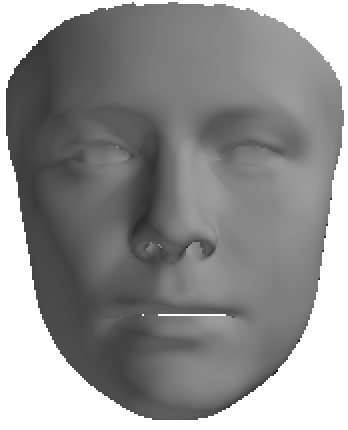
\includegraphics[width=\textwidth]{face_flow/images/contour_snapping/original_3d_model_mean}
        \caption{Mean}\label{subfig:face_flow_original_3d_mean}
    \end{subfigure} \hfill
    \begin{subfigure}[b]{0.23\textheight}
        \centering
        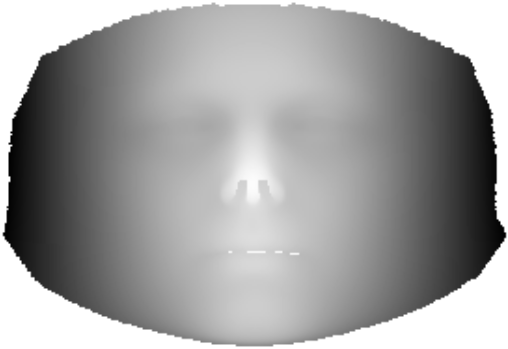
\includegraphics[width=\textwidth]{face_flow/images/contour_snapping/cylindrically_unwrapped}
        \caption{Cylindrically Unwrapped Mean}\label{subfig:face_flow_cylin_unwrap}
    \end{subfigure} \hfill
    \begin{subfigure}[b]{0.135\textheight}
        \centering
        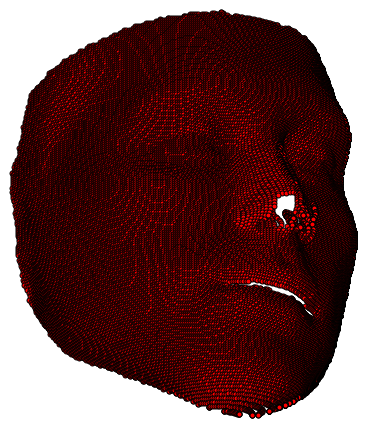
\includegraphics[width=\textwidth]{face_flow/images/contour_snapping/example_instance_high}
        \caption{High Resolution}\label{subfig:face_flow_instance_high}
    \end{subfigure} \hfill
    \begin{subfigure}[b]{0.13\textheight}
        \centering
        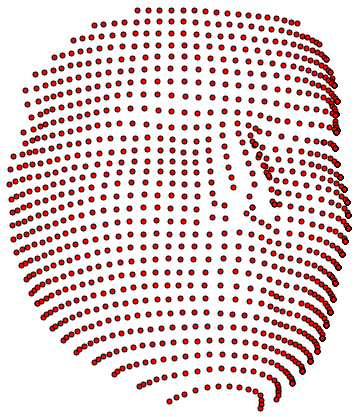
\includegraphics[width=\textwidth]{face_flow/images/contour_snapping/example_instance_low}
        \caption{Low resolution}\label{subfig:face_flow_instance_low}
    \end{subfigure}
    \hspace*{\fill}
    \caption{The model construction pipeline for the 2D deformation basis based
             on the 3D statistical model. Top row shows both the cylindrically 
             unwrapped 2D atlas and the original model mean in 3D. Bottom row
             shows a high and low resolution re-sampled instance of the rendered
             3D model.}
\label{fig:face_flow_3d_model_instance}
\end{figure}
%%%%%%%%%%%%%%%%%%%%%%%%%%%%%%%%%%%%%%%%%%%%%%%%%%%%%%%%%%%%%%%%%%%%%%%%%%%%%%%%

\textbf{3D Statistical Model.}
Although the 2D deformation basis learnt from optical flow yields a plausible
set of deformations for human faces, it does have a number of disadvantages.
Firstly, computing optical flow in the presence of large out-of-plane rotations,
such as the turning of a head, is a clear violation of the optical flow assumption
of the trajectory of a visible pixel. Therefore, incorporating pose into the
sequences makes computing the initial flows accurately a difficult process.
Furthermore, even in the case where reasonable flow can be computed for a 
sequence containing head rotations\footnote{As shown by \citet{garg2013dense}},
computing correspondences between different sequences becomes challenging
as the piecewise warping procedure above does not generalise well across large
poses. This is in part due to the difficulty of estimating sparse landmarks
in the presence of large poses and the artefacts caused by the piecewise warping
procedure from pose back to neutral.
To work around this, we propose to render an expressive 3D statistical model
under various expressions and poses and use the 2D projected positions
to describe our deformation basis. 

The main difficulty with using a 3D statistical model, such as that of
\citet{paysan20093d} or \citet{booth2016lsfm}, to construct a 2D
deformation basis is how to deal with self occlusions. These are not present when
building a model from optical flow as optical flow cannot model such 3D rotations.
These self-occlusions are an issue as when the face rotates around the yaw axis 
(left-right out-of-plane rotation) the far side of the face becomes occluded
by the near side. Naively projecting the 3D points causes the points on the far
side to become coincident with those on the nearside which will cause artefacts
when sampling pixels for the reference frame. An example of this issue
is given in \cref{fig:face_flow_pose_example} where it is shown that highly
salient regions such as the eye may be duplicated. This is a challenge for 
performing alignment as regions such as the eye provide strong texture cues and
thus these artefacts will heavily bias the recovered correspondences. To combat
this, we borrow from previous works that modify the projections to be more
consistent with the occluding contour~\cite{Zhu:2015ur,zhu2015high,hassner2015effective}.
Following \citet{zhu2015high} we assume the face to be approximately cylindrical and
cylindrically unwrap the face to construct a 2D atlas. The cylindrical unwrapping
of a point ${[x, y, z]}^T$ is given by the following mapping:
%%%%%%%%%%%%%%%%%%%
\begin{equation}
    \begin{aligned}
        \tilde{x} &\leftarrow r \theta \\
        \tilde{y} &\leftarrow y \\
        \tilde{z} &\leftarrow d
    \end{aligned}
\end{equation}
%%%%%%%%%%%%%%%%%%%
where $d = \sqrt{x^2 + y^2} - r$,
$\theta = \arctan{\left(\frac{x}{z}\right)}$ and $r$ is the provided radius 
specifying how wide the cyldinder is. Here we assume we discard the z
coordinate in order to yield a 2D atlas.
We then re-sample the mean mesh by rendering it into the area constructed by the
cylindrical unwrapping. An example of a the cylindrically unwrapped atlas is given
in \cref{subfig:face_flow_cylin_unwrap}. 
This cylindrically unwrapped atlas has two functions: firstly it
allows simple construction of a multi-scale model by interpolating the vertices 
when they are rendered into the atlas. This is demonstrated by the high
and low resolution figures given in 
\cref{subfig:face_flow_instance_high,subfig:face_flow_instance_low}. Secondly,
it allows a simple method of snapping any vertices that are occluded back
onto the occluding contour. By first removing any in-plane rotation, the
visibility mask can be used to trace occluded pixels back to their nearest
non-occluded vertex position. For example, \cref{subfig:face_flow_snapped_contour}
shows where all the occluded vertices of \cref{subfig:face_flow_occluded_vis_mask}
are snapped to for the input image of \cref{subfig:face_flow_occluded_input}.
Note that \cref{subfig:face_flow_snapped_contour} has been rotated back
``upright''. The effect of this sampling can be seen in
\cref{subfig:face_flow_snapped_sampling} where we can see that the snapped
vertices are no longer coincident with the eye region. After the snapping of
occluded pixels back to the contour, the in-plane rotation can be reapplied.
%%%%%%%%%%%%%%%%%%%%%%%%%%%%%%%%%%%%%%%%%%%%%%%%%%%%%%%%%%%%%%%%%%%%%%%%%%%%%%%%
\begin{figure}[t]
    \centering
    \hspace*{\fill}
    \begin{subfigure}[b]{0.2\textheight}
        \centering
        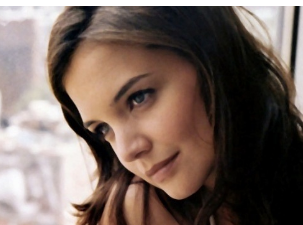
\includegraphics[width=\textwidth]{face_flow/images/contour_snapping/posed_head}
        \caption{Original Image~\cite{sagonas2013300}}\label{subfig:face_flow_occluded_input}
    \end{subfigure} \hfill
    \begin{subfigure}[b]{0.2\textheight}
        \centering
        
\includegraphics[width=\textwidth]{face_flow/images/contour_snapping/posed_visibility_mask}
        \caption{Visibility Mask}\label{subfig:face_flow_occluded_vis_mask}
    \end{subfigure} \hfill
    \begin{subfigure}[b]{0.2\textheight}
        \centering
        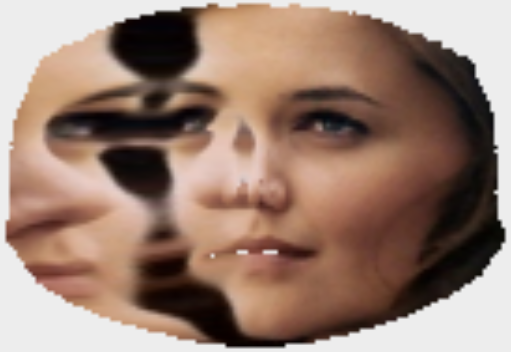
\includegraphics[width=\textwidth]{face_flow/images/contour_snapping/sampled_no_snapping}
        \caption{Naive Sampling}\label{subfig:face_flow_occluded_naive}
    \end{subfigure}
    \hspace*{\fill}
    \caption{An example of the effect the occluded points have on sampling the
             reference texture for the input in
             \cref{subfig:face_flow_occluded_input}. The visibility mask in
             \cref{subfig:face_flow_occluded_vis_mask} shows the occluded
             vertices as black and the naive sampling is shown in
             \cref{subfig:face_flow_occluded_naive}. Note how the eye is
             duplicated by the occluded points.}
\label{fig:face_flow_pose_example}
\end{figure}
%%%%%%%%%%%%%%%%%%%%%%%%%%%%%%%%%%%%%%%%%%%%%%%%%%%%%%%%%%%%%%%%%%%%%%%%%%%%%%%%

Given this new cylindrically unwrapped mesh we propose to sample
instances of the 3D statistical model, rotate them in 3D and then project them
into 2D using a scaled orthographic projection. As discussed, some vertices
will be occluded and these are snapped to the occluding contour. Finally, a
barycentric coordinate mapping from the original mesh to the cylindrically
unwrapped mesh is used in order to displace the mean vertices of the cylindrically
unwrapped mesh according the instance of the 3D model. Many renderings of this
kind are produced and from these 2D shapes we construct a 2D deformation basis
that jointly describes pose, identity and expression.
%%%%%%%%%%%%%%%%%%%%%%%%%%%%%%%%%%%%%%%%%%%%%%%%%%%%%%%%%%%%%%%%%%%%%%%%%%%%%%%%
\begin{figure}[t]
    \centering
    \hspace*{\fill}
    \begin{subfigure}[b]{0.23\textwidth}
        \centering
        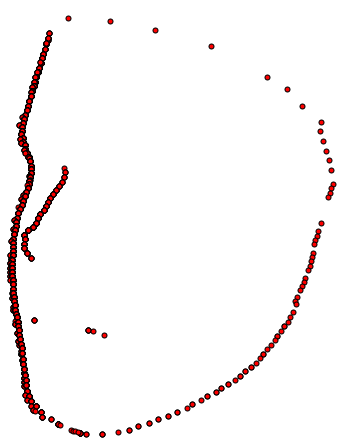
\includegraphics[width=\textwidth]{face_flow/images/contour_snapping/posed_snapped_contour}
        \caption{Snapped Vertices}\label{subfig:face_flow_snapped_contour}
    \end{subfigure} \hfill
    \begin{subfigure}[b]{0.4\textwidth}
        \centering
        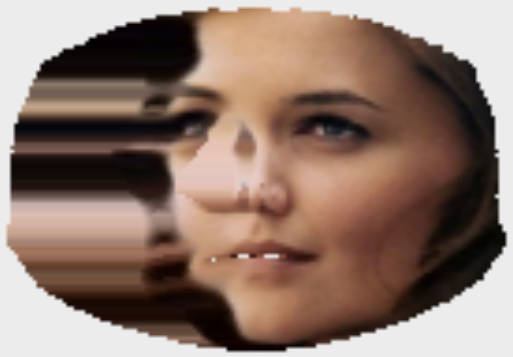
\includegraphics[width=\textwidth]{face_flow/images/contour_snapping/sampled_snapping}
        \caption{Occluded Contour Sampled}\label{subfig:face_flow_snapped_sampling}
    \end{subfigure}
    \hspace*{\fill}
    \caption{\cref{subfig:face_flow_snapped_contour} shows the vertices that
             been snapped to occluding contours. Note this includes areas such
             as the nose. \cref{subfig:face_flow_snapped_sampling} shows an
             example of sampling the texture of
             \cref{subfig:face_flow_occluded_input} with the occluding contour
             snapped mesh.}
\label{fig:face_flow_snapping_example}
\end{figure}
%%%%%%%%%%%%%%%%%%%%%%%%%%%%%%%%%%%%%%%%%%%%%%%%%%%%%%%%%%%%%%%%%%%%%%%%%%%%%%%%

%%%%%%%%%%%%%%%%%%%%%%%%%%%%%%%%%%%%%%%%%%%%%%%%%%%%%%%%%%%%%%%%%%%%%%%%%%%%%%%%
% \begin{landscape}
% \thispagestyle{footeronly}
% \setlength{\tabcolsep}{1pt}
% \begin{figure}[t]
%     \centering
%     \begin{tabular}{ccccccccc}
%            & Frame & Ground Truth & FF LR & FF FR & MFSF & LDOF & EPICFlow & SIFTFlow \\ \vspace{-0.3cm}
%         16 & \framerowsynth{nonoccluded}{16}   \\ \vspace{-0.3cm}
%         54 & \framerowsynth{nonoccluded}{54}    \\ \vspace{-0.3cm}
%         139 & \framerowsynth{nonoccluded}{139} \\
%         233 & \framerowsynth{nonoccluded}{233}
%     \end{tabular}
%     \caption{Example endpoint results for the original synthetic sequence 
%              without any outliers. Each row shows a different 
%              frame of the 280 frame synthetic sequence (Frame 16, 54, 139 and 
%              233 from top to bottom)}
% \label{fig:synthetic_no_occl_examples}
% \end{figure}
% \setlength{\tabcolsep}{6pt}
% \end{landscape}
%%%%%%%%%%%%%%%%%%%%%%%%%%%%%%%%%%%%%%%%%%%%%%%%%%%%%%%%%%%%%%%%%%%%%%%%%%%%%%%%
%%%%%%%%%%%%%%%%%%%%%%%%%%%%%%%%%%%%%%%%%%%%%%%%%%%%%%%%%%%%%%%%%%%%%%%%%%%%%%%%
% \begin{landscape}
% \thispagestyle{footeronly}
% \setlength{\tabcolsep}{1pt}
% \begin{figure}[t]
%     \centering
%     \begin{tabular}{ccccccccc}
%            & Frame & Ground Truth & FF LR & FF FR & MFSF & LDOF & EPICFlow & SIFTFlow \\ \vspace{-0.3cm}
%         16 & \framerowsynth{illumination}{16}    \\ \vspace{-0.3cm}
%         54 & \framerowsynth{illumination}{54}    \\ \vspace{-0.3cm}
%         139 & \framerowsynth{illumination}{139}  \\
%         233 & \framerowsynth{illumination}{233}
%     \end{tabular}
%     \caption{Example endpoint results for the synthetic sequence including
%              illumination variation. Each row shows a different frame of the
%              280 frame synthetic sequence (Frame 16, 54, 139 and 233 from top
%              to bottom)}
% \label{fig:synthetic_illum_examples}
% \end{figure}
% \setlength{\tabcolsep}{6pt}
% \end{landscape}
%%%%%%%%%%%%%%%%%%%%%%%%%%%%%%%%%%%%%%%%%%%%%%%%%%%%%%%%%%%%%%%%%%%%%%%%%%%%%%%%
%%%%%%%%%%%%%%%%%%%%%%%%%%%%%%%%%%%%%%%%%%%%%%%%%%%%%%%%%%%%%%%%%%%%%%%%%%%%%%%%
% \begin{landscape}
% \thispagestyle{footeronly}
% \setlength{\tabcolsep}{1pt}
% \begin{figure}[t]
%     \centering
%     \begin{tabular}{ccccccccc}
%            & Frame & Ground Truth & FF LR & FF FR & MFSF & LDOF & EPICFlow & SIFTFlow \\ \vspace{-0.3cm}
%         16 & \framerowsynth{illumination_occlusion}{16}    \\ \vspace{-0.3cm}
%         54 & \framerowsynth{illumination_occlusion}{54}    \\ \vspace{-0.3cm}
%         139 & \framerowsynth{illumination_occlusion}{139}  \\
%         233 & \framerowsynth{illumination_occlusion}{233}
%     \end{tabular}
%     \caption{Example endpoint results for the synthetic sequence including
%              illumination and occlusion variation. Each row shows a different 
%              frame of the 280 frame synthetic sequence (Frame 16, 54, 139 and 
%              233 from top to bottom)}
% \label{fig:synthetic_illum_occl_examples}
% \end{figure}
% \setlength{\tabcolsep}{6pt}
% \end{landscape}
%%%%%%%%%%%%%%%%%%%%%%%%%%%%%%%%%%%%%%%%%%%%%%%%%%%%%%%%%%%%%%%%%%%%%%%%%%%%%%%%
%%%%%%%%%%%%%%%%%%%%%%%%%%%%%%%%%%%%%%%%%%%%%%%%%%%%%%%%%%%%%%%%%%%%%%%%%%%%%%%%
\section{Experiments}\label{sec:face_flow_experiments}
%%%%%%%%%%%%%%%%%%%%%%%%%%%%%%%%%%%%%%%%%%%%%%%%%%%%%%%%%%%%%%%%%%%%%%%%%%%%%%%%
In this section, we describe the set of qualitative and quantitative experiments
that we conducted in order to demonstrate the effectiveness of our proposed algorithm,
Face Flow. In order to verify that our method is competitive with the state-of-the-art,
we compared against the methods of
\citet{garg2013variational} (denoted MFSF),
\citet{revaud2015epicflow} (denoted EPICFlow),
\citet{liu2011sift} (denoted SIFTFlow) and the large displacement
optical method of \citet{brox2011large} (denoted LDOF). We also provide two
formulations of our method, one which enforces the low-rank constraint on the coefficients
and one which does not. The latter corresponds to the choice of $\lambda=k$.
We denote these two methods Face Flow Low-Rank (LR) and Face Flow
Full-Rank (FR). This self evaluation is particularly useful for demonstrating the importance
and effectiveness of the low-rank constraint for multi-frame facial flow.

To effectively evaluate Face Flow, we propose a novel ground truth dataset formed
from facial motion capture data~\cite{zhang2004spacetime}. The sequence that we
evaluate must be in correspondence and ideally contain an interesting
sequence of deformations. Performance capture data is ideal for this purpose, as
it is necessarily in correspondence and often deals with actors portraying
scripted, emotional content. We also evaluate face flow on a realistic sequence
portraying a number of common issues in facial videos, including motion blur
and occlusions. Please see the supplementary material for
video examples of the sequences and further results.
%%%%%%%%%%%%%%%%%%%%%%%%%%%%%%%%%%%%%%%%%%%%%%%%%%%%%%%%%%%%%%%%%%%%%%%%%%%%%%%%
\subsection{Practical Deformation Basis Construction}\label{subsec:face_flow_experiments_basis}
%%%%%%%%%%%%%%%%%%%%%%%%%%%%%%%%%%%%%%%%%%%%%%%%%%%%%%%%%%%%%%%%%%%%%%%%%%%%%%%%
%%%%%%%%%%%%%%%%%%%%%%%%%%%%%%%%%%%%%%%%
\setlength{\tabcolsep}{2pt}
\begin{figure}
    \centering
    \resizebox{\textwidth}{!}{%
    \begin{tabular}{cccccc}
    Mean &  PC 1 & PC 2 & PC 3 & PC 4 & PC 5 \\
    \multirow{2}{*}{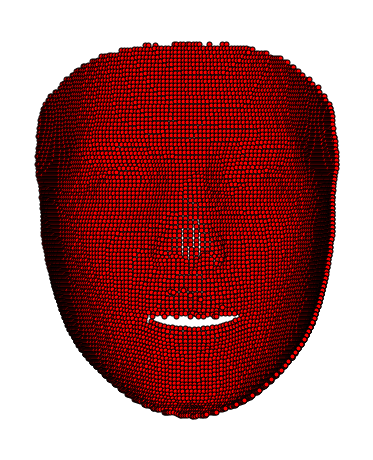
\includegraphics[valign=m,scale=0.16]{face_flow/images/3d_pca_basis/mean}} &  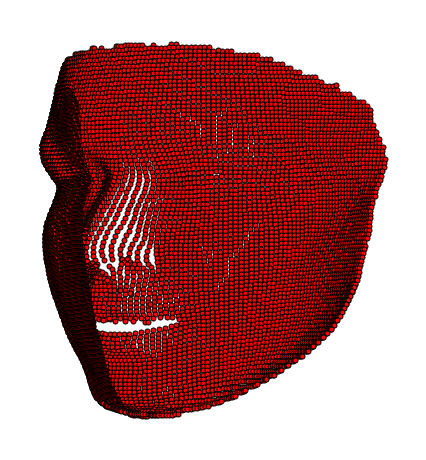
\includegraphics[valign=m,scale=0.16]{face_flow/images/3d_pca_basis/0_plus2} & 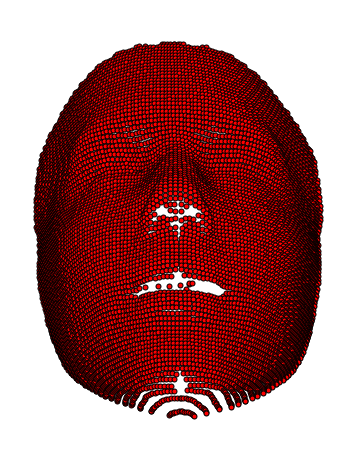
\includegraphics[valign=m,scale=0.16]{face_flow/images/3d_pca_basis/1_plus2} & 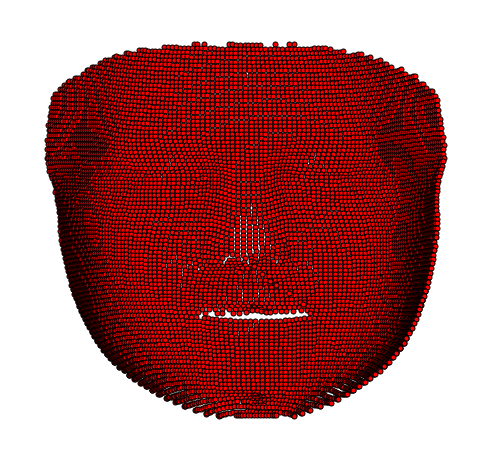
\includegraphics[valign=m,scale=0.16]{face_flow/images/3d_pca_basis/2_plus2} & 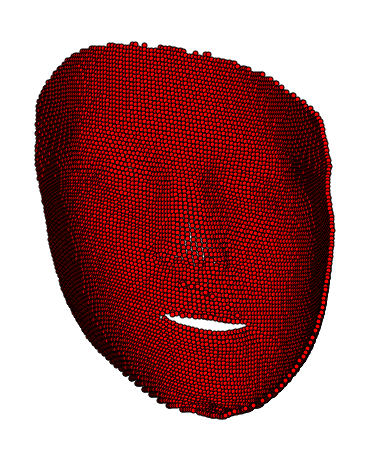
\includegraphics[valign=m,scale=0.16]{face_flow/images/3d_pca_basis/3_plus2} & 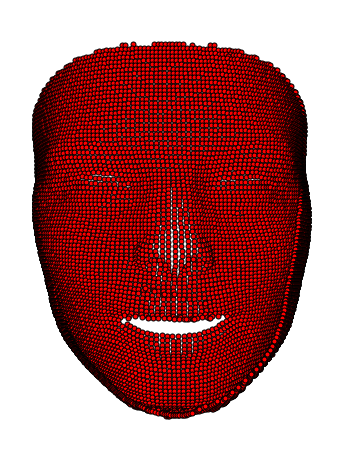
\includegraphics[valign=m,scale=0.16]{face_flow/images/3d_pca_basis/4_plus2} \\
     & 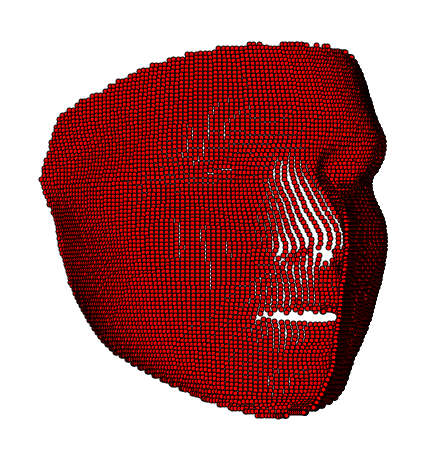
\includegraphics[valign=m,scale=0.16]{face_flow/images/3d_pca_basis/0_minus2} & 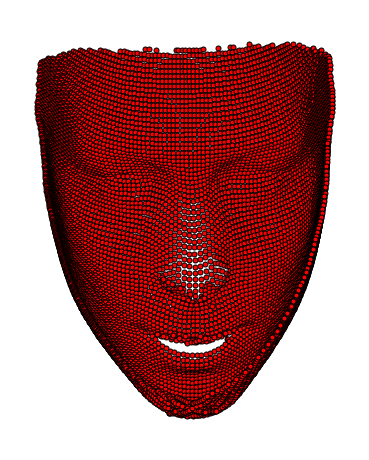
\includegraphics[valign=m,scale=0.16]{face_flow/images/3d_pca_basis/1_minus2} & 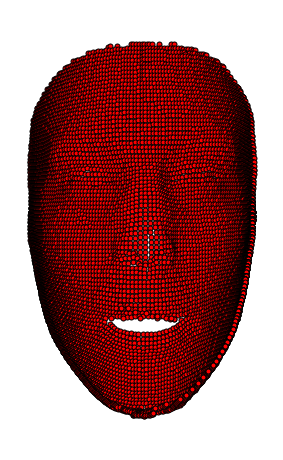
\includegraphics[valign=m,scale=0.16]{face_flow/images/3d_pca_basis/2_minus2} & 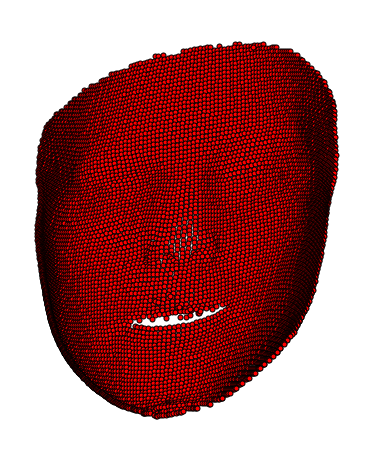
\includegraphics[valign=m,scale=0.16]{face_flow/images/3d_pca_basis/3_minus2} & 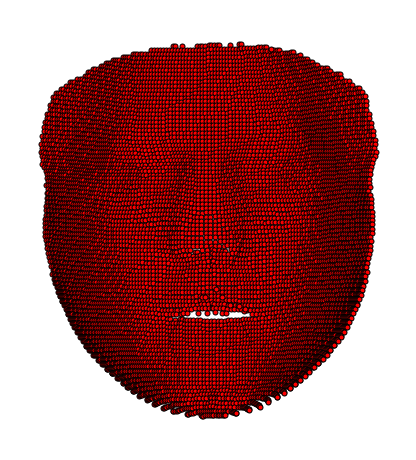
\includegraphics[valign=m,scale=0.16]{face_flow/images/3d_pca_basis/4_minus2}
    \end{tabular}%
    }
    \caption{The PCA basis of facial deformation learnt from the 
             3D LSFM~\cite{booth2016lsfm} model as described in 
             \cref{subsec:face_flow_experiments_basis}. The top and bottoms rows
             show the principals components for $\pm 2 \sigma$ respectively.}
\label{fig:face_flow_3d_pca_basis}
\end{figure}
\setlength{\tabcolsep}{6pt}
%%%%%%%%%%%%%%%%%%%%%%%%%%%%%%%%%%%%%%%%
%%%%%%%%%%%%%%%%%%%%%%%%%%%%%%%%%%%%%%%%
\setlength{\tabcolsep}{2pt}
\begin{figure}
    \centering
    \resizebox{\textwidth}{!}{%
    \begin{tabular}{cccccc}
    Mean &  PC 1 & PC 2 & PC 3 & PC 4 & PC 5 \\
    \multirow{2}{*}{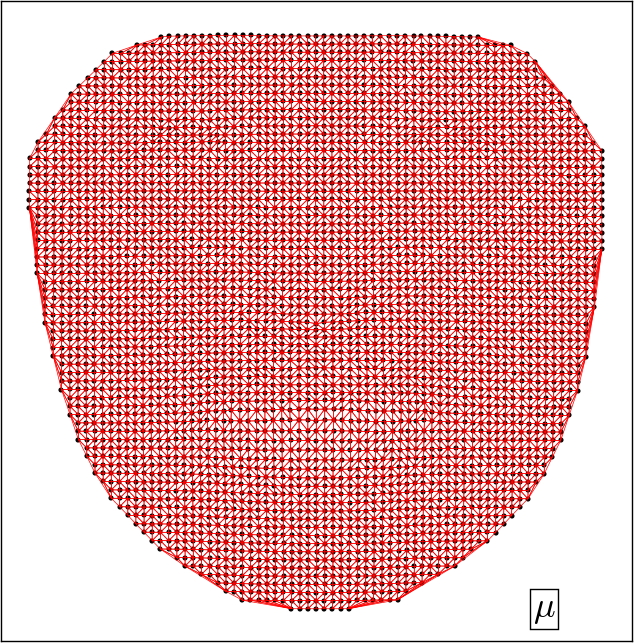
\includegraphics[valign=m,scale=0.16]{face_flow/images/of_pca_basis/mean}} &  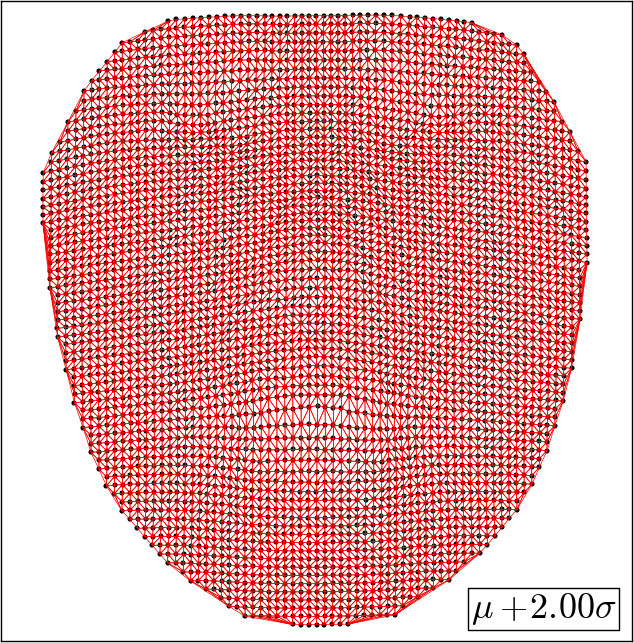
\includegraphics[valign=m,scale=0.16]{face_flow/images/of_pca_basis/0_plus2} & 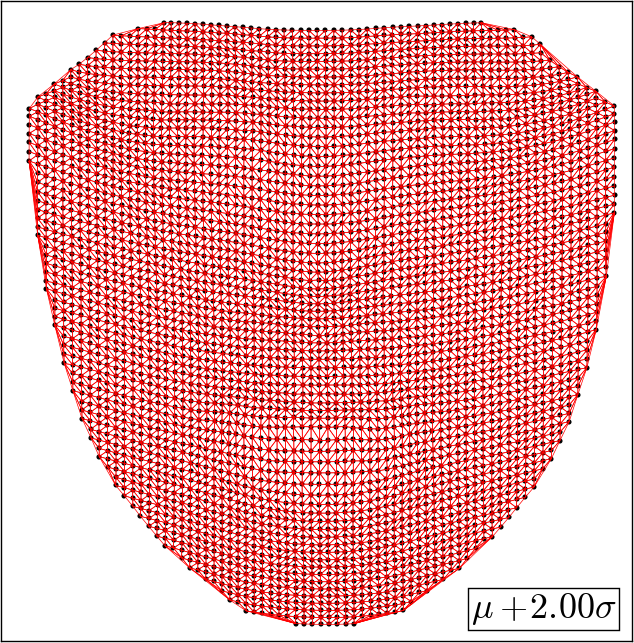
\includegraphics[valign=m,scale=0.16]{face_flow/images/of_pca_basis/1_plus2} & 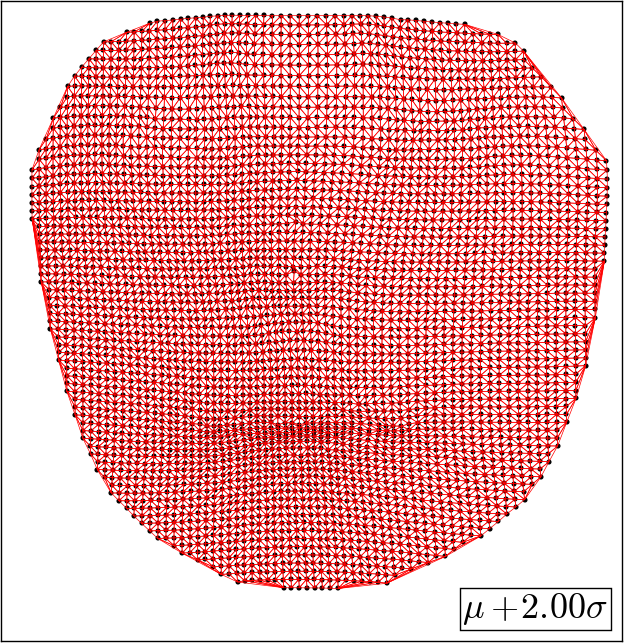
\includegraphics[valign=m,scale=0.16]{face_flow/images/of_pca_basis/2_plus2} & 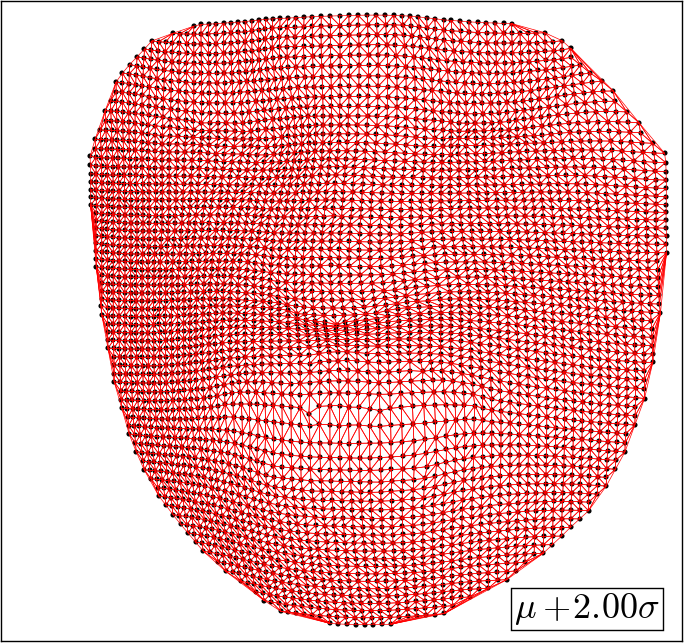
\includegraphics[valign=m,scale=0.16]{face_flow/images/of_pca_basis/3_plus2} & 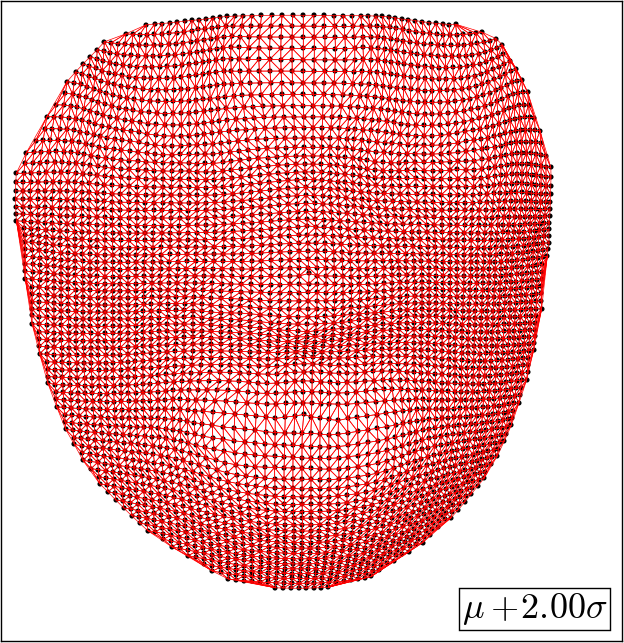
\includegraphics[valign=m,scale=0.16]{face_flow/images/of_pca_basis/4_plus2} \\
     & 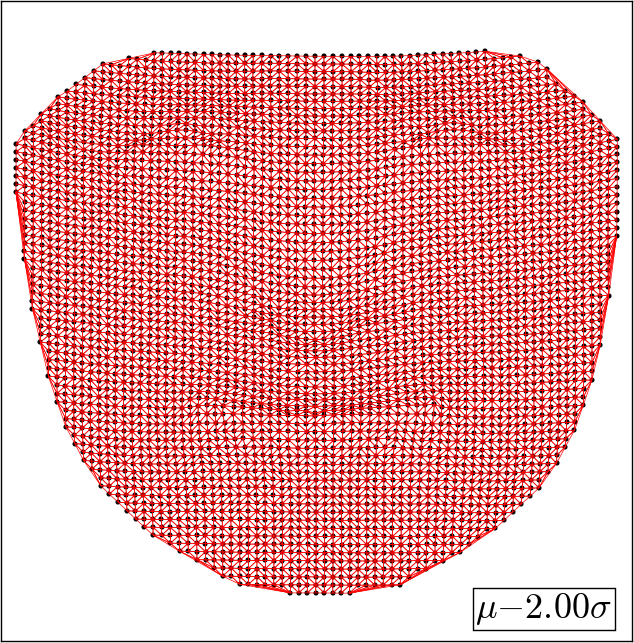
\includegraphics[valign=m,scale=0.16]{face_flow/images/of_pca_basis/0_minus2} & 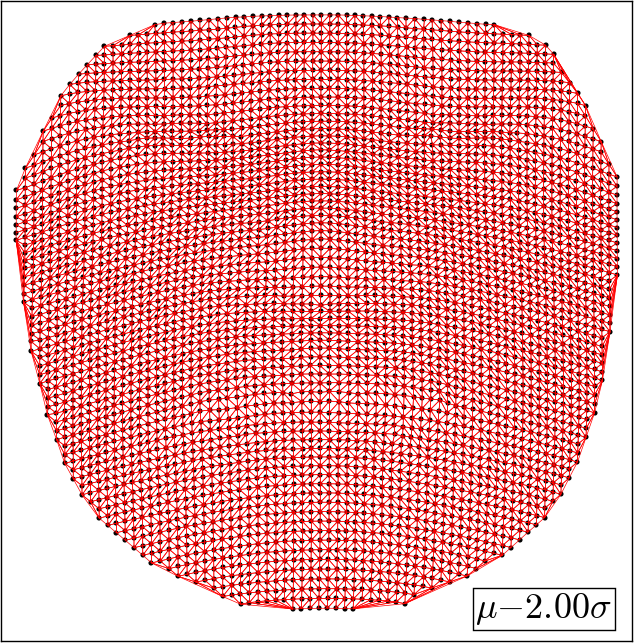
\includegraphics[valign=m,scale=0.16]{face_flow/images/of_pca_basis/1_minus2} & 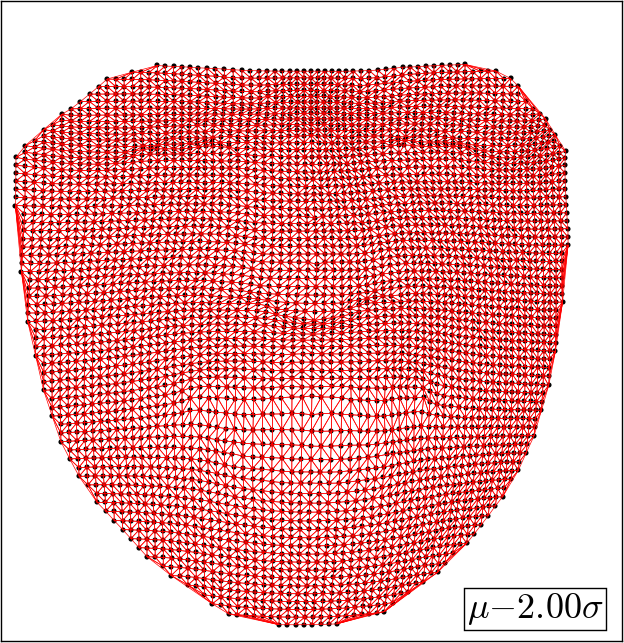
\includegraphics[valign=m,scale=0.16]{face_flow/images/of_pca_basis/2_minus2} & 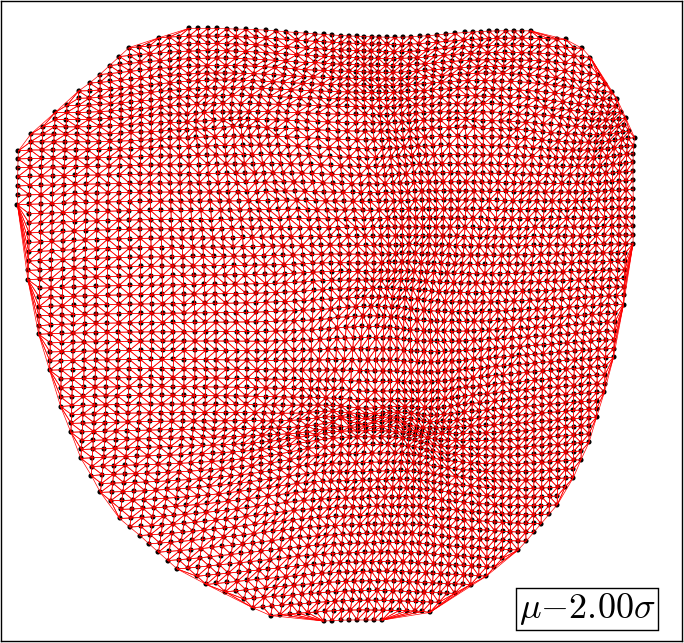
\includegraphics[valign=m,scale=0.16]{face_flow/images/of_pca_basis/3_minus2} & 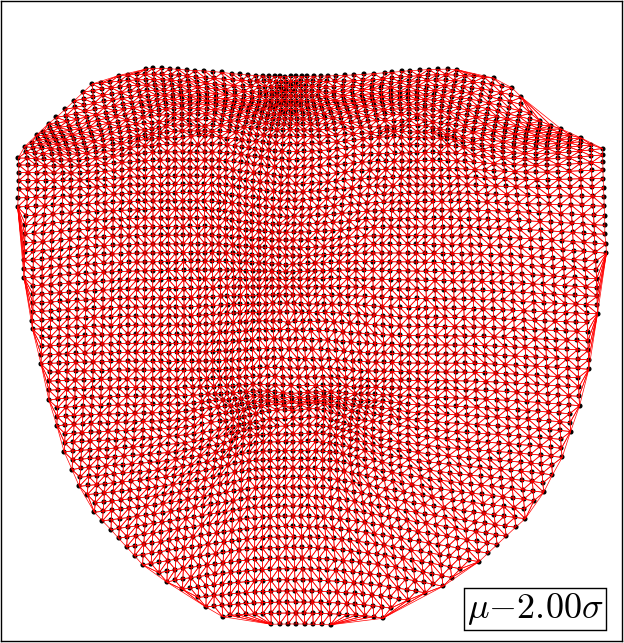
\includegraphics[valign=m,scale=0.16]{face_flow/images/of_pca_basis/4_minus2}
    \end{tabular}%
    }
    \caption{The PCA basis of facial deformation learnt from the 
             BU4D~\cite{yin2008high} database as described in 
             \cref{subsec:face_flow_experiments_basis}. The top and bottoms rows
             show the principals components for $\pm 2 \sigma$ respectively.}
\label{fig:face_flow_of_pca_basis}
\end{figure}
\setlength{\tabcolsep}{6pt}
%%%%%%%%%%%%%%%%%%%%%%%%%%%%%%%%%%%%%%%%
Our facial deformation basis is built by applying MFSF multi-frame optical flow method
\footnote{Code publicly available at https://bitbucket.org/troussos/mfsf/} of \citet{garg2013variational} on
the facial expression database BU4D~\cite{yin2008high}. We chose this database due
to the large range of expression present and the fact that is captured at a high
frame rate, which is ideal for the technique of \citet{garg2013variational}. However, in order
to further improve the performance of \citet{garg2013variational}, we augmented the energy
to include an extra quadratic landmark constraint. This landmark constraint
takes a similar form to the landmark constraint proposed in this paper, and was
found to improve the results considerably in sequences that displayed particularly
expressive emotion, such as surprise.

The BU4D database consists of 102 subjects displaying 6 canonical expression,
from neutral to the apex of the emotion. We selected a neutral frame for every
sequence and used this as the reference frame for the method of \citet{garg2013variational}.
After computing trajectories for each sequence,
we constructed a reference frame for our deformation basis using the mean
of the neutral images we selected previously. We then applied principal
component analysis (PCA) to learn the linear deformation model as described in 
\cref{sec:face_flow_learning_deformation}.
Experimentally, we found that $k=20$ principal components of
non-rigid deformation accounts for $~95\%$ of the variance.
We note that the BU4D-FE data shows frontal faces and thus our model does not capture out-of-plane
rotation. However, there is no practical reason that our PCA basis could not capture
this kind of deformation.

In order to improve the robustness of our algorithm, we adopt a pseudo coarse-to-fine
strategy for basis construction and create three bases of increasing scale. This is also
commonly employed within optical algorithms to improve robustness. In all of the following experiments,
the feature descriptor employed is the dense SIFT feature.
%%%%%%%%%%%%%%%%%%%%%%%%%%%%%%%%%%%%%%%%%%%%%%%%%%%%%%%%%%%%%%%%%%%%%%%%%%%%%%%%
\subsection{Motion Capture Data}\label{subsec:face_flow_experiments_mocap}
%%%%%%%%%%%%%%%%%%%%%%%%%%%%%%%%%%%%%%%%%%%%%%%%%%%%%%%%%%%%%%%%%%%%%%%%%%%%%%%%
In this experiment, we use the performance capture dataset provided by \citet{zhang2004spacetime}
to generate three novel ground truth sequences consisting of 280 frames. This ground truth is provided by rendering
the sequence of meshes in a fixed pose, which yields both a texture and a set of vertices
in the scene. These vertices can then be used in order simply calculate flow for the face
throughout the image.

As mentioned, we rendered three sets of texture, all with the same underlying geometry,
to provide evidence of the robustness of Face Flow to challenging conditions. In the first
sequence, we rendered unmodified textures. This is a baseline
in order to show the performance of state-of-the-art methods for facial data. Since
our basis is trained using the output from~\cite{garg2013variational}, we do not expect to
outperform other optical flow techniques on this sequence. The second sequence
was rendered by rendering a periodically moving light source around the face. This
is challenging for the data term and helps to demonstrate the
robustness of our chosen feature descriptor. The final sequence is highly challenging. It contains
the periodic illumination variation from the previous sequence and also an artificial
occlusion in the form of a smoothly translating hand.

In order to initialise our Face Flow algorithm, we manually annotated the first frame
as the reference frame. To obtain an initial estimate of the coefficient
matrix $\mathbf{C}$, the landmark constraint quadratic term is solved, which
provides a reasonable estimate of the initial shape. Once solved in the reference frame,
this initialisation was propagated across every frame in the sequence. The landmark constraint
was otherwise not utilised in this experiment.

To evaluate the performance of the methods, we computed the root mean squared
error of the endpoints (RMSE), shown in Table~\ref{tbl:synthetic}. As expected
Face Flow does not outperform state-of-the-art methods in the original un-tampered
sequence. However, in the more interesting case of the illumination variation
and occlusion sequences, our Face Flow method with low-rank constraint (Face Flow LR),
performs the best. We also note that the low-rank method of our technique significantly
outperforms the full-rank version, particularly in the occluded sequence. An example
set of endpoints is given in Figure~\ref{fig:synthetic_illum_examples}. Note how
the face deformation is well localised and unlikely to undergo any gross deformations
due to being constrained by a statistical basis.

Finally, to provide evidence as to the stability of our algorithm, and the effect
of the low-rank constraint on the outcome of the sequence, we present Figure~\ref{fig:per_frame_error}.
This figure shows the mean per-frame endpoint error across the sequence. The Face Flow
methods are given by the blue and green lines. Note how stable the Face Flow LR method is,
particularly when compared to the Face Flow FR method. We believe this effectively
demonstrates the positive effect enforcing soft temporal consistency can have.
%%%%%%%%%%%%%%%%%%%%%%%%%%%%%%%%%%%%%%%%%%%%%%%%%%%%%%%%%%%%%%%%%%%%%%%%%%%%%%%%
\subsection{Real Sequence}\label{subsec:face_flow_experiments_real}
%%%%%%%%%%%%%%%%%%%%%%%%%%%%%%%%%%%%%%%%%%%%%%%%%%%%%%%%%%%%%%%%%%%%%%%%%%%%%%%%
For this experiment, we provide results on a real sequence consisting
of 150 frames of a young woman watching a video. In this sequence, she reacts
negatively and clearly presents discomfort by touching her face and shifting
in her seat. This amounts to challenging variation in the sequence, including
occlusions from her hand and motion blur from movement. In this sequence,
we also provide evidence as to the benefit of incorporating the landmark constraint. The sequence was
automatically landmarked using~\cite{kazemi2014one}, then our method was initialised with
these landmarks for every frame. We also used the landmarks for the quadratic penalizer term.
As Figure~\ref{fig:real_examples} shows, Face Flow LR performs very well in this sequence. In particular,
we note that our method is very robust to the presence of occlusions, aided by the sparse
landmarks provided by~\cite{kazemi2014one}. We also provide Table~\ref{tbl:run_times}
which demonstrates that Face Flow is an order of magnitude more efficient than
the other considered methods for this sequence.
%%%%%%%%%%%%%%%%%%%%%%%%%%%%%%%%%%%%%%%%%%%%%%%%%%%%%%%%%%%%%%%%%%%%%%%%%%%%%%%%
\begin{table}[t]
    \centering
    \begin{tabular}{cccccc}
                                                     \toprule
FF LR & FF FR & MFSF & LDOF & EPICFlow & SIFTFlow \\ \toprule
1.4   & 0.5   & 20   & 15   & $\sim$50 & 15       \\ \bottomrule
    \end{tabular}
    \caption{Run times \textit{per frame (in seconds)} for the 150 frame
             sequence shown in Figure~\ref{fig:real_examples}. Images are
             $640\times480$. Performed on an Intel Xeon E5--1650 3.20GHz
             (32GB RAM). All times are approximate and averaged over multiple
             runs. EPICFlow times are dominated by
             DEEPMatching~\cite{weinzaepfel2013deepflow} ($~48$s).}
\label{tbl:run_times}
\end{table}
%%%%%%%%%%%%%%%%%%%%%%%%%%%%%%%%%%%%%%%%%%%%%%%%%%%%%%%%%%%%%%%%%%%%%%%%%%%%%%%%
%%%%%%%%%%%%%%%%%%%%%%%%%%%%%%%%%%%%%%%%%%%%%%%%%%%%%%%%%%%%%%%%%%%%%%%%%%%%%%%%
\begin{table}
    \centering
    \begin{tabular}{lrrrrrr}
                                                                                                                                       \toprule
         & \multicolumn{2}{c}{Original}            & \multicolumn{2}{c}{Illum.}              & \multicolumn{2}{c}{Ilum.+Occ.}          \\
         & {\scriptsize RMSE} & {\scriptsize AE95} & {\scriptsize RMSE} & {\scriptsize AE95} & {\scriptsize RMSE} & {\scriptsize AE95} \\ \toprule
FF LR    & 2.95               & 5.52               & {\bf 3.56}         & {\bf 6.63}         & {\bf 4.48}         & {\bf 8.47}         \\
FF FR    & 3.24               & 6.01               & 3.76               & 7.02               & 5.83               & 11.50              \\
MFSF     & 1.73               & 3.20               & 6.33               & 13.68              & 8.25               & 17.30              \\
LDOF     & {\bf 1.56}         & {\bf 2.79}         & 4.84               & 9.98               & 6.54               & 11.44              \\
EPICFlow & 1.66               & 3.25               & 4.02               & 9.61               & 5.15               & 11.61              \\
SIFTF    & 2.65               & 5.15               & 4.89               & 11.81              & 11.82              & 23.05              \\ \bottomrule
    \end{tabular}
    \caption{RMSE and 95\% average endpoint error for the synthetic data.}
\label{tbl:synthetic}
\end{table}
%%%%%%%%%%%%%%%%%%%%%%%%%%%%%%%%%%%%%%%%%%%%%%%%%%%%%%%%%%%%%%%%%%%%%%%%%%%%%%%%
%%%%%%%%%%%%%%%%%%%%%%%%%%%%%%%%%%%%%%%%%%%%%%%%%%%%%%%%%%%%%%%%%%%%%%%%%%%%%%%%
\begin{figure}[t]
    \centering
    \begin{subfigure}{6in}
        \centering
        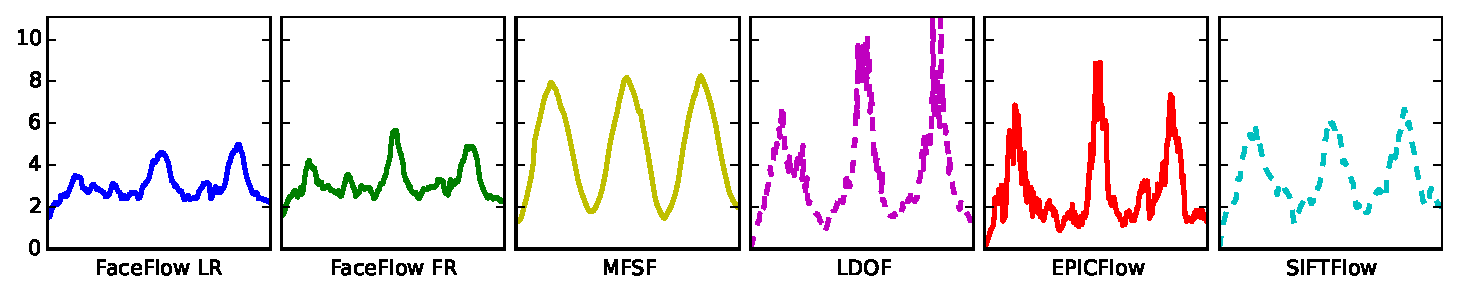
\includegraphics[width=\textwidth]{face_flow/images/synthetic/frame_error_5_flat}
    \end{subfigure}  \\
    \begin{subfigure}{6in}
        \centering
        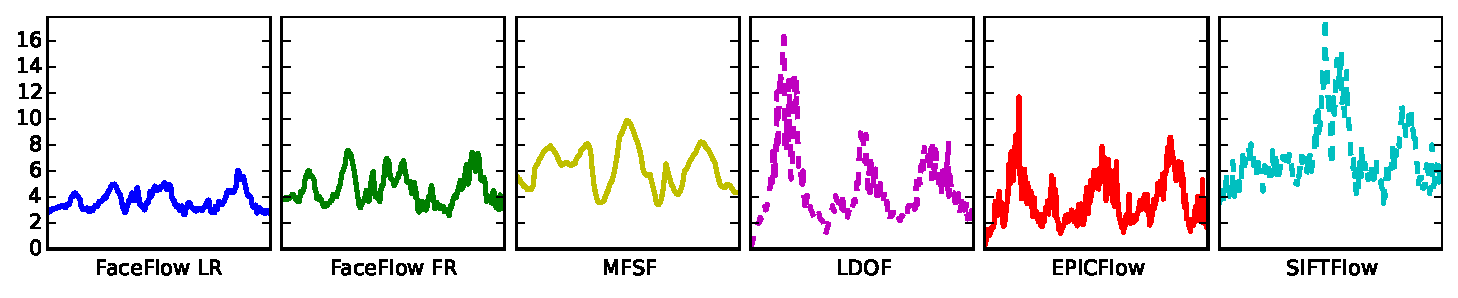
\includegraphics[width=\textwidth]{face_flow/images/synthetic/frame_error_6_flat}
    \end{subfigure}
    \caption{The average endpoint error calculated for each frame of the mocap
             sequence. Vertical axis is average endpoint error, horizontal is
             frame number. Top row is the illumination sequence, bottom row is
             illumination + occlusion.}
\label{fig:per_frame_error}
\end{figure}
%%%%%%%%%%%%%%%%%%%%%%%%%%%%%%%%%%%%%%%%%%%%%%%%%%%%%%%%%%%%%%%%%%%%%%%%%%%%%%%%
%%%%%%%%%%%%%%%%%%%%%%%%%%%%%%%%%%%%%%%%%%%%%%%%%%%%%%%%%%%%%%%%%%%%%%%%%%%%%%%%
\begin{landscape}
\thispagestyle{footeronly}
\newcommand{\framerowreal}[1]{%
\adjustbox{valign=m,vspace=1pt}{\includegraphics[width=4.5cm,height=3.45cm]{face_flow/images/real/#1_ff_dsift_sequence}} &
\adjustbox{valign=m,vspace=1pt}{\includegraphics[width=4.5cm,height=3.45cm]{face_flow/images/real/#1_mfsf}}              &
\adjustbox{valign=m,vspace=1pt}{\includegraphics[width=4.5cm,height=3.45cm]{face_flow/images/real/#1_ldof}}              &
\adjustbox{valign=m,vspace=1pt}{\includegraphics[width=4.5cm,height=3.45cm]{face_flow/images/real/#1_epicflow}}          &
\adjustbox{valign=m,vspace=1pt}{\includegraphics[width=4.5cm,height=3.45cm]{face_flow/images/real/#1_siftflow}}
}

\setlength{\tabcolsep}{1pt}
\begin{figure}[t]
    \centering
    \begin{tabular}{cccccc}
           & Face Flow LR & MFSF & LDOF & EPICFlow & SIFTFlow \\ \vspace{-0.1cm}
        15 & \framerowreal{15}                                \\ \vspace{-0.1cm}
        21 & \framerowreal{21}                                \\ \vspace{-0.1cm}
       119 & \framerowreal{119}
    \end{tabular}
    \caption{Results on real data. Here, we incorporate the landmark constraint
             and thus do not give results for Face Flow FR.}
\label{fig:real_examples}
\end{figure}
\setlength{\tabcolsep}{6pt}
\end{landscape}
% %%%%%%%%%%%%%%%%%%%%%%%%%%%%%%%%%%%%%%%%%%%%%%%%%%%%%%%%%%%%%%%%%%%%%%%%%%%%%%%%

%%%%%%%%%%%%%%%%%%%%%%%%%%%%%%%%%%%%%%%%%%%%%%%%%%%%%%%%%%%%%%%%%%%%%%%%%%%%%%%%
\section{Conclusion}\label{sec:conclusion}
%%%%%%%%%%%%%%%%%%%%%%%%%%%%%%%%%%%%%%%%%%%%%%%%%%%%%%%%%%%%%%%%%%%%%%%%%%%%%%%%
We presented an optical flow method that incorporates a dense
basis of facial shape. We evaluated our method on a ground truth motion capture
sequence and demonstrated that our proposed algorithm, Face Flow, outperforms
other state-of-the-art optical flow methods. In particular, the introduction
of a low-rank constraint yields a robust multi-frame optical flow technique.
As future work, we intend to investigate a more complex dataset that would enable
Face Flow to model out-of-plane rotations.
}
%%%%%%%%%%%%%%%%%%%%%%%%%%%%%%%%%%%%%%%%%%%%%%%%%%%%%%%%%%%%%%%%%%%%%%%%%%%%%%%%
\stopcontents[chapters]
%%%%%%%%%%%%%%%%%%%%%%%%%%%%%%%%%%%%%%%%%%%%%%%%%%%%%%%%%%%%%%%%%%%%%%%%%%%%%%%%
